\documentclass[fullpage,twocolumn]{article} % For LaTeX2e
\usepackage{times}
% \iclrfinalcopy

\addtolength{\oddsidemargin}{-.1in}
	\addtolength{\evensidemargin}{-.1in}
	\addtolength{\textwidth}{.2in}

	\addtolength{\topmargin}{-.875in}
	\addtolength{\textheight}{1.75in}

\usepackage{fancyhdr}
 
\pagestyle{fancy}
\fancyhf{}
\rhead{Under constrction}
\lhead{Draft}
\rfoot{Page \thepage}
 
%\usepackage{draftwatermark}
%\SetWatermarkText{Draft}
%\SetWatermarkScale{2}
%\SetWatermarkColor[rgb]{1,.9,.9}

\usepackage{amsmath,amssymb} 
% Optional math commands from https://github.com/goodfeli/dlbook_notation.
%%%%% NEW MATH DEFINITIONS %%%%%

\usepackage{amsmath,amsfonts,bm}

% Mark sections of captions for referring to divisions of figures
\newcommand{\figleft}{{\em (Left)}}
\newcommand{\figcenter}{{\em (Center)}}
\newcommand{\figright}{{\em (Right)}}
\newcommand{\figtop}{{\em (Top)}}
\newcommand{\figbottom}{{\em (Bottom)}}
\newcommand{\captiona}{{\em (a)}}
\newcommand{\captionb}{{\em (b)}}
\newcommand{\captionc}{{\em (c)}}
\newcommand{\captiond}{{\em (d)}}

% Highlight a newly defined term
\newcommand{\newterm}[1]{{\bf #1}}


% Figure reference, lower-case.
\def\figref#1{figure~\ref{#1}}
% Figure reference, capital. For start of sentence
\def\Figref#1{Figure~\ref{#1}}
\def\twofigref#1#2{figures \ref{#1} and \ref{#2}}
\def\quadfigref#1#2#3#4{figures \ref{#1}, \ref{#2}, \ref{#3} and \ref{#4}}
% Section reference, lower-case.
\def\secref#1{section~\ref{#1}}
% Section reference, capital.
\def\Secref#1{Section~\ref{#1}}
% Reference to two sections.
\def\twosecrefs#1#2{sections \ref{#1} and \ref{#2}}
% Reference to three sections.
\def\secrefs#1#2#3{sections \ref{#1}, \ref{#2} and \ref{#3}}
% Reference to an equation, lower-case.
\def\eqref#1{equation~\ref{#1}}
% Reference to an equation, upper case
\def\Eqref#1{Equation~\ref{#1}}
% A raw reference to an equation---avoid using if possible
\def\plaineqref#1{\ref{#1}}
% Reference to a chapter, lower-case.
\def\chapref#1{chapter~\ref{#1}}
% Reference to an equation, upper case.
\def\Chapref#1{Chapter~\ref{#1}}
% Reference to a range of chapters
\def\rangechapref#1#2{chapters\ref{#1}--\ref{#2}}
% Reference to an algorithm, lower-case.
\def\algref#1{algorithm~\ref{#1}}
% Reference to an algorithm, upper case.
\def\Algref#1{Algorithm~\ref{#1}}
\def\twoalgref#1#2{algorithms \ref{#1} and \ref{#2}}
\def\Twoalgref#1#2{Algorithms \ref{#1} and \ref{#2}}
% Reference to a part, lower case
\def\partref#1{part~\ref{#1}}
% Reference to a part, upper case
\def\Partref#1{Part~\ref{#1}}
\def\twopartref#1#2{parts \ref{#1} and \ref{#2}}

\def\ceil#1{\lceil #1 \rceil}
\def\floor#1{\lfloor #1 \rfloor}
\def\1{\bm{1}}
\newcommand{\train}{\mathcal{D}}
\newcommand{\valid}{\mathcal{D_{\mathrm{valid}}}}
\newcommand{\test}{\mathcal{D_{\mathrm{test}}}}

\def\eps{{\epsilon}}


% Random variables
\def\reta{{\textnormal{$\eta$}}}
\def\ra{{\textnormal{a}}}
\def\rb{{\textnormal{b}}}
\def\rc{{\textnormal{c}}}
\def\rd{{\textnormal{d}}}
\def\re{{\textnormal{e}}}
\def\rf{{\textnormal{f}}}
\def\rg{{\textnormal{g}}}
\def\rh{{\textnormal{h}}}
\def\ri{{\textnormal{i}}}
\def\rj{{\textnormal{j}}}
\def\rk{{\textnormal{k}}}
\def\rl{{\textnormal{l}}}
% rm is already a command, just don't name any random variables m
\def\rn{{\textnormal{n}}}
\def\ro{{\textnormal{o}}}
\def\rp{{\textnormal{p}}}
\def\rq{{\textnormal{q}}}
\def\rr{{\textnormal{r}}}
\def\rs{{\textnormal{s}}}
\def\rt{{\textnormal{t}}}
\def\ru{{\textnormal{u}}}
\def\rv{{\textnormal{v}}}
\def\rw{{\textnormal{w}}}
\def\rx{{\textnormal{x}}}
\def\ry{{\textnormal{y}}}
\def\rz{{\textnormal{z}}}

% Random vectors
\def\rvepsilon{{\mathbf{\epsilon}}}
\def\rvtheta{{\mathbf{\theta}}}
\def\rva{{\mathbf{a}}}
\def\rvb{{\mathbf{b}}}
\def\rvc{{\mathbf{c}}}
\def\rvd{{\mathbf{d}}}
\def\rve{{\mathbf{e}}}
\def\rvf{{\mathbf{f}}}
\def\rvg{{\mathbf{g}}}
\def\rvh{{\mathbf{h}}}
\def\rvu{{\mathbf{i}}}
\def\rvj{{\mathbf{j}}}
\def\rvk{{\mathbf{k}}}
\def\rvl{{\mathbf{l}}}
\def\rvm{{\mathbf{m}}}
\def\rvn{{\mathbf{n}}}
\def\rvo{{\mathbf{o}}}
\def\rvp{{\mathbf{p}}}
\def\rvq{{\mathbf{q}}}
\def\rvr{{\mathbf{r}}}
\def\rvs{{\mathbf{s}}}
\def\rvt{{\mathbf{t}}}
\def\rvu{{\mathbf{u}}}
\def\rvv{{\mathbf{v}}}
\def\rvw{{\mathbf{w}}}
\def\rvx{{\mathbf{x}}}
\def\rvy{{\mathbf{y}}}
\def\rvz{{\mathbf{z}}}

% Elements of random vectors
\def\erva{{\textnormal{a}}}
\def\ervb{{\textnormal{b}}}
\def\ervc{{\textnormal{c}}}
\def\ervd{{\textnormal{d}}}
\def\erve{{\textnormal{e}}}
\def\ervf{{\textnormal{f}}}
\def\ervg{{\textnormal{g}}}
\def\ervh{{\textnormal{h}}}
\def\ervi{{\textnormal{i}}}
\def\ervj{{\textnormal{j}}}
\def\ervk{{\textnormal{k}}}
\def\ervl{{\textnormal{l}}}
\def\ervm{{\textnormal{m}}}
\def\ervn{{\textnormal{n}}}
\def\ervo{{\textnormal{o}}}
\def\ervp{{\textnormal{p}}}
\def\ervq{{\textnormal{q}}}
\def\ervr{{\textnormal{r}}}
\def\ervs{{\textnormal{s}}}
\def\ervt{{\textnormal{t}}}
\def\ervu{{\textnormal{u}}}
\def\ervv{{\textnormal{v}}}
\def\ervw{{\textnormal{w}}}
\def\ervx{{\textnormal{x}}}
\def\ervy{{\textnormal{y}}}
\def\ervz{{\textnormal{z}}}

% Random matrices
\def\rmA{{\mathbf{A}}}
\def\rmB{{\mathbf{B}}}
\def\rmC{{\mathbf{C}}}
\def\rmD{{\mathbf{D}}}
\def\rmE{{\mathbf{E}}}
\def\rmF{{\mathbf{F}}}
\def\rmG{{\mathbf{G}}}
\def\rmH{{\mathbf{H}}}
\def\rmI{{\mathbf{I}}}
\def\rmJ{{\mathbf{J}}}
\def\rmK{{\mathbf{K}}}
\def\rmL{{\mathbf{L}}}
\def\rmM{{\mathbf{M}}}
\def\rmN{{\mathbf{N}}}
\def\rmO{{\mathbf{O}}}
\def\rmP{{\mathbf{P}}}
\def\rmQ{{\mathbf{Q}}}
\def\rmR{{\mathbf{R}}}
\def\rmS{{\mathbf{S}}}
\def\rmT{{\mathbf{T}}}
\def\rmU{{\mathbf{U}}}
\def\rmV{{\mathbf{V}}}
\def\rmW{{\mathbf{W}}}
\def\rmX{{\mathbf{X}}}
\def\rmY{{\mathbf{Y}}}
\def\rmZ{{\mathbf{Z}}}

% Elements of random matrices
\def\ermA{{\textnormal{A}}}
\def\ermB{{\textnormal{B}}}
\def\ermC{{\textnormal{C}}}
\def\ermD{{\textnormal{D}}}
\def\ermE{{\textnormal{E}}}
\def\ermF{{\textnormal{F}}}
\def\ermG{{\textnormal{G}}}
\def\ermH{{\textnormal{H}}}
\def\ermI{{\textnormal{I}}}
\def\ermJ{{\textnormal{J}}}
\def\ermK{{\textnormal{K}}}
\def\ermL{{\textnormal{L}}}
\def\ermM{{\textnormal{M}}}
\def\ermN{{\textnormal{N}}}
\def\ermO{{\textnormal{O}}}
\def\ermP{{\textnormal{P}}}
\def\ermQ{{\textnormal{Q}}}
\def\ermR{{\textnormal{R}}}
\def\ermS{{\textnormal{S}}}
\def\ermT{{\textnormal{T}}}
\def\ermU{{\textnormal{U}}}
\def\ermV{{\textnormal{V}}}
\def\ermW{{\textnormal{W}}}
\def\ermX{{\textnormal{X}}}
\def\ermY{{\textnormal{Y}}}
\def\ermZ{{\textnormal{Z}}}

% Vectors
\def\vzero{{\bm{0}}}
\def\vone{{\bm{1}}}
\def\vmu{{\bm{\mu}}}
\def\vtheta{{\bm{\theta}}}
\def\va{{\bm{a}}}
\def\vb{{\bm{b}}}
\def\vc{{\bm{c}}}
\def\vd{{\bm{d}}}
\def\ve{{\bm{e}}}
\def\vf{{\bm{f}}}
\def\vg{{\bm{g}}}
\def\vh{{\bm{h}}}
\def\vi{{\bm{i}}}
\def\vj{{\bm{j}}}
\def\vk{{\bm{k}}}
\def\vl{{\bm{l}}}
\def\vm{{\bm{m}}}
\def\vn{{\bm{n}}}
\def\vo{{\bm{o}}}
\def\vp{{\bm{p}}}
\def\vq{{\bm{q}}}
\def\vr{{\bm{r}}}
\def\vs{{\bm{s}}}
\def\vt{{\bm{t}}}
\def\vu{{\bm{u}}}
\def\vv{{\bm{v}}}
\def\vw{{\bm{w}}}
\def\vx{{\bm{x}}}
\def\vy{{\bm{y}}}
\def\vz{{\bm{z}}}

% Elements of vectors
\def\evalpha{{\alpha}}
\def\evbeta{{\beta}}
\def\evepsilon{{\epsilon}}
\def\evlambda{{\lambda}}
\def\evomega{{\omega}}
\def\evmu{{\mu}}
\def\evpsi{{\psi}}
\def\evsigma{{\sigma}}
\def\evtheta{{\theta}}
\def\eva{{a}}
\def\evb{{b}}
\def\evc{{c}}
\def\evd{{d}}
\def\eve{{e}}
\def\evf{{f}}
\def\evg{{g}}
\def\evh{{h}}
\def\evi{{i}}
\def\evj{{j}}
\def\evk{{k}}
\def\evl{{l}}
\def\evm{{m}}
\def\evn{{n}}
\def\evo{{o}}
\def\evp{{p}}
\def\evq{{q}}
\def\evr{{r}}
\def\evs{{s}}
\def\evt{{t}}
\def\evu{{u}}
\def\evv{{v}}
\def\evw{{w}}
\def\evx{{x}}
\def\evy{{y}}
\def\evz{{z}}

% Matrix
\def\mA{{\bm{A}}}
\def\mB{{\bm{B}}}
\def\mC{{\bm{C}}}
\def\mD{{\bm{D}}}
\def\mE{{\bm{E}}}
\def\mF{{\bm{F}}}
\def\mG{{\bm{G}}}
\def\mH{{\bm{H}}}
\def\mI{{\bm{I}}}
\def\mJ{{\bm{J}}}
\def\mK{{\bm{K}}}
\def\mL{{\bm{L}}}
\def\mM{{\bm{M}}}
\def\mN{{\bm{N}}}
\def\mO{{\bm{O}}}
\def\mP{{\bm{P}}}
\def\mQ{{\bm{Q}}}
\def\mR{{\bm{R}}}
\def\mS{{\bm{S}}}
\def\mT{{\bm{T}}}
\def\mU{{\bm{U}}}
\def\mV{{\bm{V}}}
\def\mW{{\bm{W}}}
\def\mX{{\bm{X}}}
\def\mY{{\bm{Y}}}
\def\mZ{{\bm{Z}}}
\def\mBeta{{\bm{\beta}}}
\def\mPhi{{\bm{\Phi}}}
\def\mLambda{{\bm{\Lambda}}}
\def\mSigma{{\bm{\Sigma}}}

% Tensor
\DeclareMathAlphabet{\mathsfit}{\encodingdefault}{\sfdefault}{m}{sl}
\SetMathAlphabet{\mathsfit}{bold}{\encodingdefault}{\sfdefault}{bx}{n}
\newcommand{\tens}[1]{\bm{\mathsfit{#1}}}
\def\tA{{\tens{A}}}
\def\tB{{\tens{B}}}
\def\tC{{\tens{C}}}
\def\tD{{\tens{D}}}
\def\tE{{\tens{E}}}
\def\tF{{\tens{F}}}
\def\tG{{\tens{G}}}
\def\tH{{\tens{H}}}
\def\tI{{\tens{I}}}
\def\tJ{{\tens{J}}}
\def\tK{{\tens{K}}}
\def\tL{{\tens{L}}}
\def\tM{{\tens{M}}}
\def\tN{{\tens{N}}}
\def\tO{{\tens{O}}}
\def\tP{{\tens{P}}}
\def\tQ{{\tens{Q}}}
\def\tR{{\tens{R}}}
\def\tS{{\tens{S}}}
\def\tT{{\tens{T}}}
\def\tU{{\tens{U}}}
\def\tV{{\tens{V}}}
\def\tW{{\tens{W}}}
\def\tX{{\tens{X}}}
\def\tY{{\tens{Y}}}
\def\tZ{{\tens{Z}}}


% Graph
\def\gA{{\mathcal{A}}}
\def\gB{{\mathcal{B}}}
\def\gC{{\mathcal{C}}}
\def\gD{{\mathcal{D}}}
\def\gE{{\mathcal{E}}}
\def\gF{{\mathcal{F}}}
\def\gG{{\mathcal{G}}}
\def\gH{{\mathcal{H}}}
\def\gI{{\mathcal{I}}}
\def\gJ{{\mathcal{J}}}
\def\gK{{\mathcal{K}}}
\def\gL{{\mathcal{L}}}
\def\gM{{\mathcal{M}}}
\def\gN{{\mathcal{N}}}
\def\gO{{\mathcal{O}}}
\def\gP{{\mathcal{P}}}
\def\gQ{{\mathcal{Q}}}
\def\gR{{\mathcal{R}}}
\def\gS{{\mathcal{S}}}
\def\gT{{\mathcal{T}}}
\def\gU{{\mathcal{U}}}
\def\gV{{\mathcal{V}}}
\def\gW{{\mathcal{W}}}
\def\gX{{\mathcal{X}}}
\def\gY{{\mathcal{Y}}}
\def\gZ{{\mathcal{Z}}}

% Sets
\def\sA{{\mathbb{A}}}
\def\sB{{\mathbb{B}}}
\def\sC{{\mathbb{C}}}
\def\sD{{\mathbb{D}}}
% Don't use a set called E, because this would be the same as our symbol
% for expectation.
\def\sF{{\mathbb{F}}}
\def\sG{{\mathbb{G}}}
\def\sH{{\mathbb{H}}}
\def\sI{{\mathbb{I}}}
\def\sJ{{\mathbb{J}}}
\def\sK{{\mathbb{K}}}
\def\sL{{\mathbb{L}}}
\def\sM{{\mathbb{M}}}
\def\sN{{\mathbb{N}}}
\def\sO{{\mathbb{O}}}
\def\sP{{\mathbb{P}}}
\def\sQ{{\mathbb{Q}}}
\def\sR{{\mathbb{R}}}
\def\sS{{\mathbb{S}}}
\def\sT{{\mathbb{T}}}
\def\sU{{\mathbb{U}}}
\def\sV{{\mathbb{V}}}
\def\sW{{\mathbb{W}}}
\def\sX{{\mathbb{X}}}
\def\sY{{\mathbb{Y}}}
\def\sZ{{\mathbb{Z}}}

% Entries of a matrix
\def\emLambda{{\Lambda}}
\def\emA{{A}}
\def\emB{{B}}
\def\emC{{C}}
\def\emD{{D}}
\def\emE{{E}}
\def\emF{{F}}
\def\emG{{G}}
\def\emH{{H}}
\def\emI{{I}}
\def\emJ{{J}}
\def\emK{{K}}
\def\emL{{L}}
\def\emM{{M}}
\def\emN{{N}}
\def\emO{{O}}
\def\emP{{P}}
\def\emQ{{Q}}
\def\emR{{R}}
\def\emS{{S}}
\def\emT{{T}}
\def\emU{{U}}
\def\emV{{V}}
\def\emW{{W}}
\def\emX{{X}}
\def\emY{{Y}}
\def\emZ{{Z}}
\def\emSigma{{\Sigma}}

% entries of a tensor
% Same font as tensor, without \bm wrapper
\newcommand{\etens}[1]{\mathsfit{#1}}
\def\etLambda{{\etens{\Lambda}}}
\def\etA{{\etens{A}}}
\def\etB{{\etens{B}}}
\def\etC{{\etens{C}}}
\def\etD{{\etens{D}}}
\def\etE{{\etens{E}}}
\def\etF{{\etens{F}}}
\def\etG{{\etens{G}}}
\def\etH{{\etens{H}}}
\def\etI{{\etens{I}}}
\def\etJ{{\etens{J}}}
\def\etK{{\etens{K}}}
\def\etL{{\etens{L}}}
\def\etM{{\etens{M}}}
\def\etN{{\etens{N}}}
\def\etO{{\etens{O}}}
\def\etP{{\etens{P}}}
\def\etQ{{\etens{Q}}}
\def\etR{{\etens{R}}}
\def\etS{{\etens{S}}}
\def\etT{{\etens{T}}}
\def\etU{{\etens{U}}}
\def\etV{{\etens{V}}}
\def\etW{{\etens{W}}}
\def\etX{{\etens{X}}}
\def\etY{{\etens{Y}}}
\def\etZ{{\etens{Z}}}

% The true underlying data generating distribution
\newcommand{\pdata}{p_{\rm{data}}}
% The empirical distribution defined by the training set
\newcommand{\ptrain}{\hat{p}_{\rm{data}}}
\newcommand{\Ptrain}{\hat{P}_{\rm{data}}}
% The model distribution
\newcommand{\pmodel}{p_{\rm{model}}}
\newcommand{\Pmodel}{P_{\rm{model}}}
\newcommand{\ptildemodel}{\tilde{p}_{\rm{model}}}
% Stochastic autoencoder distributions
\newcommand{\pencode}{p_{\rm{encoder}}}
\newcommand{\pdecode}{p_{\rm{decoder}}}
\newcommand{\precons}{p_{\rm{reconstruct}}}

\newcommand{\laplace}{\mathrm{Laplace}} % Laplace distribution

\newcommand{\E}{\mathbb{E}}
\newcommand{\Ls}{\mathcal{L}}
\newcommand{\R}{\mathbb{R}}
\newcommand{\emp}{\tilde{p}}
\newcommand{\lr}{\alpha}
\newcommand{\reg}{\lambda}
\newcommand{\rect}{\mathrm{rectifier}}
\newcommand{\softmax}{\mathrm{softmax}}
\newcommand{\sigmoid}{\sigma}
\newcommand{\softplus}{\zeta}
\newcommand{\KL}{D_{\mathrm{KL}}}
\newcommand{\Var}{\mathrm{Var}}
\newcommand{\standarderror}{\mathrm{SE}}
\newcommand{\Cov}{\mathrm{Cov}}
% Wolfram Mathworld says $L^2$ is for function spaces and $\ell^2$ is for vectors
% But then they seem to use $L^2$ for vectors throughout the site, and so does
% wikipedia.
\newcommand{\normlzero}{L^0}
\newcommand{\normlone}{L^1}
\newcommand{\normltwo}{L^2}
\newcommand{\normlp}{L^p}
\newcommand{\normmax}{L^\infty}

\newcommand{\parents}{Pa} % See usage in notation.tex. Chosen to match Daphne's book.

\DeclareMathOperator*{\argmax}{arg\,max}
\DeclareMathOperator*{\argmin}{arg\,min}

\DeclareMathOperator{\sign}{sign}
\DeclareMathOperator{\Tr}{Tr}
\let\ab\allowbreak


\usepackage{natbib}
\usepackage{hyperref}
\usepackage{url}
\usepackage{verbatim}
\usepackage{listings}
\usepackage{subcaption}
\usepackage{graphicx}
\usepackage{algorithm}
\usepackage{algpseudocode}
\usepackage{mathtools}
\usepackage{booktabs}
\usepackage{adjustbox}
\usepackage[textwidth=3cm]{todonotes}
\usepackage{tikz}
\usepackage{wrapfig}

\DeclareMathOperator*{\Oplus}{\bigoplus}

\title{Knossos: An RL compiler for AI workloads}

% Authors must not appear in the submitted version. They should be hidden
% as long as the \iclrfinalcopy macro remains commented out below.
% Non-anonymous submissions will be rejected without review.

\author{Project Knossos team, MSR Cambridge.\\Contact: Andrew Fitzgibbon, Ryota Tomioka}

% The \author macro works with any number of authors. There are two commands
% used to separate the names and addresses of multiple authors: \And and \AND.
%
% Using \And between authors leaves it to \LaTeX{} to determine where to break
% the lines. Using \AND forces a linebreak at that point. So, if \LaTeX{}
% puts 3 of 4 authors names on the first line, and the last on the second
% line, try using \AND instead of \And before the third author name.

\lstset{basicstyle=\ttfamily\footnotesize,breaklines=true, tabsize=2}

\newcommand{\fix}{\marginpar{FIX}}
\newcommand{\new}{\marginpar{NEW}}
\newcommand{\Rplus}{\protect\hspace{-.1em}\protect\raisebox{.35ex}{\smaller{\smaller\textbf{+}}}}
\def\Cpp{{C\nolinebreak[4]\hspace{-.05em}\raisebox{.4ex}{\tiny\bf ++}} }
\newcommand{\Exp}{\operatorname{E}}
\newcommand{\Vtarget}{V^\text{target}}
\newcommand{\SuccessRate}{p_\text{success}}

\newcommand{\open}{O}
\newcommand{\closed}{C}
% \newcommand{\open}{{\bm O}}
% \newcommand{\closed}{{\bm C}}

\algnewcommand{\LineComment}[1]{\State \(\triangleright\) #1}

%\iclrfinalcopy % Uncomment for camera-ready version, but NOT for submission.
\begin{document}

\maketitle

\begin{abstract}
Machine learning workloads are often expensive to train, taking weeks to converge. The current generation of frameworks relies on custom back-ends in order to achieve efficiency, making it impractical to train models on less common hardware where no such back-ends exist. Knossos builds on recent work that avoids the need for hand-written libraries, instead compiles machine learning models in much the same way one would compile other kinds of software. To make the resulting code efficient, the Knossos compiler directly optimises the abstract syntax tree of the program. We formalize program optimisation as a finite-horizon Markov Decision Process (MDP) and train an agent that performs $A^\star$ search guided by a learned value function. We show that Knossos can automatically learn optimisations that past compilers had to implement by hand. Furthermore, we demonstrate that Knossos can achieve wall time reduction compared to a hand-tuned compiler on a suite of machine learning programs, including basic linear algebra and convolutional networks.
The Knossos compiler has minimal dependencies and can be used on any architecture that supports a \Cpp toolchain. 
Since the cost model Knossos optimises can be tailored to a particular hardware architecture, the proposed approach can potentially be applied to a variety of hardware.
\end{abstract}

% or for problems that cannot be efficiently expressed in terms of tensor operations.

% Knossos uses an intermediate representation and a suite of transpilers, allowing the programmer to focus on the core task of specifying the machine learning algorithm using the full syntax of a language they know.

%Second, they require the programmer to either manually specify a computation graph using meta-programming or rely on a restricted subset of a high-level language, introducing an unnecessary level of indirection. The Knossos compiler addresses both of these issues. 


\section{Introduction}
While all software development can benefit from compilers able to produce fast code, runtime efficiency is particularity important for modern machine learning. In particular, because modern models can take weeks to train \citep{ai-and-compute}, compiler optimisations that lead to execution speed-ups are of huge value. In parallel, machine learning is being deployed on a variety of diverse devices ranging from wearables to huge clusters clusters of powerful GPUs. Since each architecture has different performance profile and requires different code optimisations, it is difficult to provide tooling that works fast on all of them.

Traditionally, the tension between performance and interoperability is resolved by machine learning frameworks \citep{paszkeAutomaticDifferentiationPyTorch2017a, abadiTensorFlowSystemLargeScale2016}, where code execution is outsourced to hardware-specific back-ends. While this approach has seen huge initial success, the cost of providing a customised back-end for each target architecture is prohibitive. Moreover, the frameworks also custom front-ends that require the programmer to specify the model being trained as a compute graph. Since the compute graph has semantics separate from the host programming language, this process is often error-prone and time-consuming. In order to address these obstacles, a new generation of tools has recently appeared that transform machine learning code using the same techniques that have been used for compiling traditional software. The need for a separate front-end API for machine learning operations is eliminated by including automatic differentiation as a first-class feature of the complied language \citep{innes2019zygote, jax}. Instead of custom back-ends, modern machine learning compilers use an intermediate representation and perform extensive code optimisations \citep{innes2019zygote, jax, merrienboerAutomaticDifferentiationML2018, weiDLVMModernCompiler2018, sotoudehISAMapperCompute2019, rotemGlowGraphLowering2018}. In addition, program optimisation is being modelled as a machine learning task itself, with the compiler learning how to perform rewrites \citep{chenLearningOptimizeTensor2018, chenTVMAutomatedEndtoEnd2018}. 

Knossos expands on this line of work. The Knossos system includes a compiler which combines efficient program optimisation with an intermediate representation (IR) designed with machine learning in mind. We formalize program optimisation as a finite-horizon Markov Decision Process (MDP), with the reward signal determined by a configurable model of the cost of executing a program. By solving this MDP, we are able to produce fast code tailor-made for any given task and architecture, without relying on backend-specific hand-written libraries. Akin to JAX \citep{jax} and Zygote \citep{innes2019zygote}, all Knossos functions are potentially differentiable, avoiding the syntactic awkwardness that arises from embedding a differentiable program in a host language. The IR can then be transpiled, allowing it to run on any platform that supports a \Cpp toolchain. This allows Knossos code to be seamlessly deployed on specialized or embedded hardware without the need of manual tuning, both for training and for deployment of models, enabling a much broader user base than competing approaches.

To our knowledge, Knossos is the first compiler that combines RL-based program optimisation, first-class support for deep learning primitives and the ability to target any architecture supporting the \Cpp toolchain. We defer detailed scope comparisons with prior work to Section \ref{sec-related-work}. We empirically demonstrate the benefits of our program optimisation in Section \ref{sec-benchmarks}, showing that Knossos was able to automatically learn \emph{loop fusion}, a type of compiler optimisation that previously had to be applied manually.

\section{Code Optimisation as a Reinforcement Learning Problem}
\label{sec-mdp-def}
We model code optimisation as a finite-horizon Markov Decision Process (MDP). An MDP is defined \citep{Puterman2014, suttonReinforcementLearningIntroduction2018} as a tuple $(S, A, T, R, H, p_0)$, where $S$ denotes the state space, $A$ denotes the action space, $T$ denotes the transition dynamics, $R$ denotes the rewards, $H$ is the maximum time budget allowed to solve the problem (the horizon) and $p_0$ is a fixed probability distribution over initial states. We provide a detailed description of the states, transitions and rewards later on this section.

\begin{figure*}[t!]
    \centering
    \begin{subfigure}{0.4\textwidth}
        \centering
        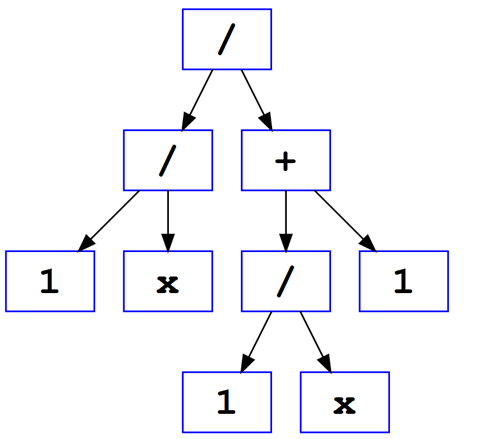
\includegraphics[height=3.2cm]{sample-expression}
        \caption{Sample arithmetic expression tree (MDP state). The tree corresponds to $\frac{1/x}{1/x + 1}$, which can be optimised to $\frac{1}{1+x}$.}  
        \label{sample-state}
    \end{subfigure}
    \begin{subfigure}{0.59\textwidth}
    \begin{center}
    \begin{minipage}{0.99\textwidth}
\begin{lstlisting}[caption=,frame=tlrb]{rewrite-rules}
(rule (add 0 e)                 e)
(rule (mul 1 e)                 e)
(rule (div (mul a b) c)         (mul (div a c) b))
(rule (mul (exp a) (exp b))     (exp (add a b)))
(rule (if p a a)                a))
(rule (apply (lam x body) arg)  (let x arg body))
(rule e                         (let x e x))
        \end{lstlisting}
        \end{minipage}
        \end{center}
        %\includegraphics[height=1.2in]{b}
        \caption{Example rewrite rules. Each rule defines a class of MDP transitions. See \ref{appendix-rewrites} for the full list of rules.}
        \label{sample-rules}
    \end{subfigure}
    \caption{The Knossos MDP: (a) State, (b) Transitions.}
\end{figure*}

\paragraph{States and transitions}
An MDP state $s=(e_s,t_s)$ consists of a Knossos program (or expression) $e\in E$ and the remaining time budget $t_s\in[0, 1,\ldots, H]$ (i.e., the number of remaining  steps), where $H$ is the maximum budget. Any state with $t_s=0$ is terminating. The initial state distribution $p_0$ models the expressions that the RL agent is likely to be asked to optimize. A sample Knossos expression is shown in Fig. \ref{sample-state}. The action set $A$ corresponds to different possible ways of rewriting the same expression (see Fig. \ref{sample-rules}). The transition function $T:S\times A\rightarrow S$ returns the next state after taking an action.
For example, the first rule in Fig. \ref{sample-rules} says that adding zero to any expression can be simplified to the expression itself. Once the action is chosen, the transition is deterministic. Because rewrite rules can be applied to different subexpressions, we specify $A$ using generic rewrite rules, which are applied by pattern matching.
%
There are over 50 rules like this -- we provide the details in \ref{appendix-rewrites}. An essential feature of the rewrites is that they do not change the meaning of the program, i.e.\ by simplifying from one expression to another we also implicitly generate a proof that the expressions are equivalent. 

\paragraph{Policies and Value Functions} The RL agent maintains a policy $\pi(a \vert s)$, which defines the probability of taking an action in state~$s$ given there are $t_s$ steps remaining till the total time budget is exhausted. A policy $\pi$ generates rollouts $\tau_\pi$. A rollout $\tau_\pi$ is defined as a sequence of states, actions and rewards obtained from the MDP $\tau_\pi = \left( s_1, a_1, r_1, s_2, a_2, r_2, \dots s_H, r_H \right )$. Since the policy $\pi$ can be stochastic, it is modelled as a random variable. The goal of RL agent is to find an optimal policy $\pi^\star = \argmax_\pi J_\pi$, which attains the best possible return. The return is defined as $J_\pi =  \Exp_{\tau_\pi} \left[ \sum_{t=0}^{t={H-1}} R(s_t, s_{t+1}) \right] $. Given a policy and the number of timesteps $t$ remaining till the end of episode, we define a value function $V(s) = \Exp_{\tau} \left[ \sum_{i=0}^{t_s-1} R(s_i, s_{i+1}) \; \Big\vert \; s_0 = s\right]$, where $t_s$ denotes the remaining time budget at state $s$. The optimal value function $V^\star$ is defined as the value function of an optimal policy $\pi^\star$.

\paragraph{Rewards and the Cost Model} 
We assume access to a function $c(s)$, which provides the \emph{cost model}, i.e.\ the computational cost of running  $e_s$, the expression represented by state $s = (e_s,t_s)$, on representative inputs. While developing a perfect cost models is theoretically impossible due to the intractability of the halting problem \citep{turing1937computable}, very good cost models exist for the particular subset of programs that compilers are asked to optimise. The ideal cost model $c_B$ would correspond to the run-time of the program on typical inputs, but evaluating costs by benchmarking is very computationally intensive. In practice, one can often find a surrogate cost function such that for most initial programs $s_0$, the state that is reachable from $s_0$ and minimizes the surrogate cost function $c$ agrees with that for the ideal cost function $c_B$, that is,
\begin{gather}
\argmin_{s\sim s_0}  c(s) = \argmin_{s\sim s_0} c_B(s),
\end{gather}
which is much easier to acquire. In other words, the cost function $c$ does not have to produce the same run-time but the same minimum over programs. We show experimentally in Section \ref{sec-benchmarks} that it is indeed possible to reduce the wall clock time of running a program by optimising such a proxy cost model. Knossos has a modular architecture, making it easy to change the cost function. This makes it possible to quickly re-tune Knossos programs for any target hardware. We stress that the formalism allows us to find optimisations even in case getting to the optimized version of the code requires using intermediate programs of higher cost (see Fig.~\ref{mnist-qualit}).

%
\begin{figure}
    \centering
    \vspace*{-2mm}
    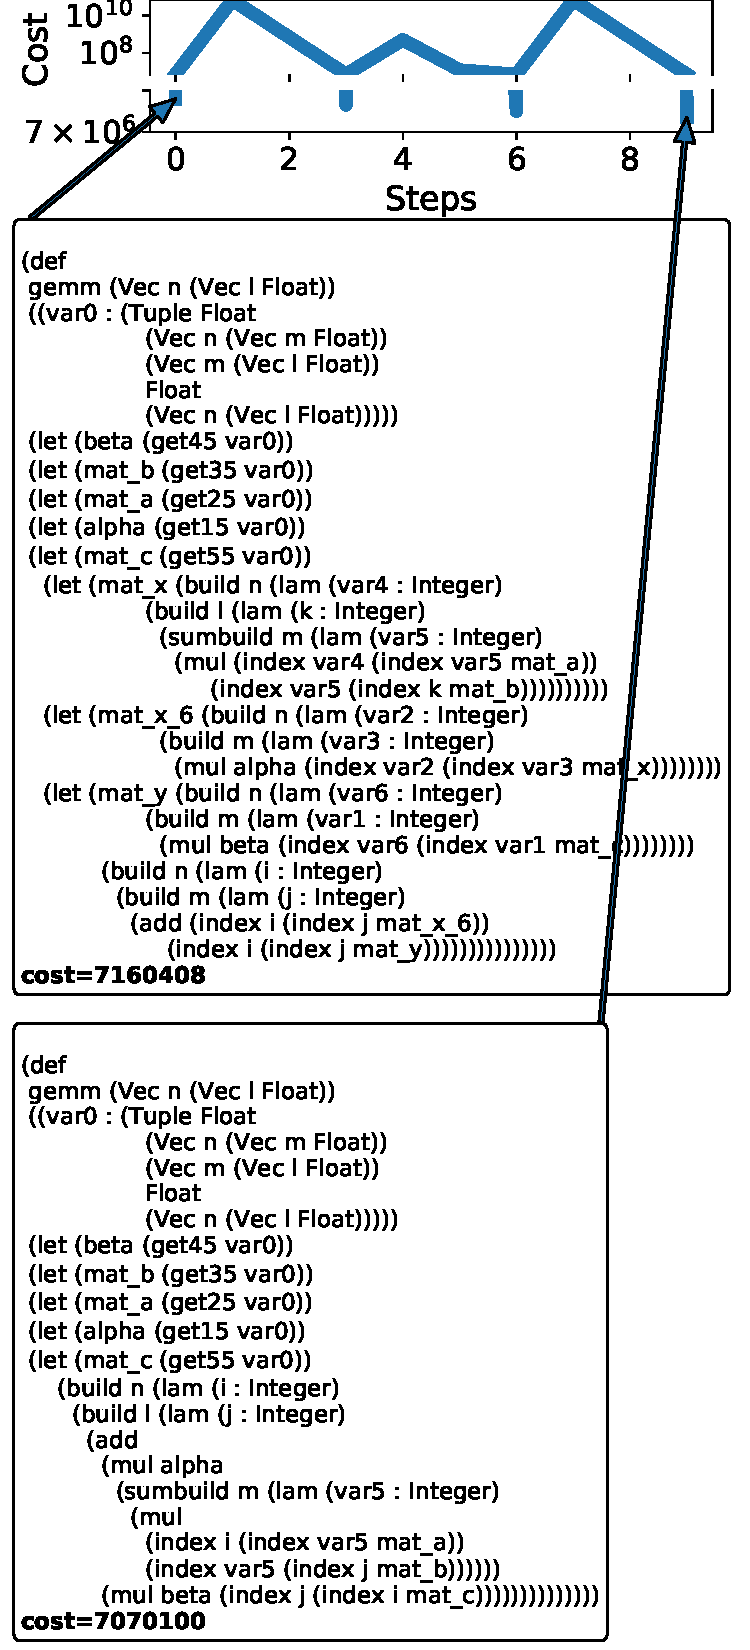
\includegraphics[width=.35\textwidth]{cost_sequence_blas.pdf}
    \caption{General Matrix Multiply (GEMM) program rewrite sequence. The initial expression was obtained from our rule-based \texttt{ksc} compiler and shown in the middle. The final expression is obtained after 10 rewriting steps and shown in the bottom.}
    \label{gemm-qualit}
\end{figure}
%



Our reward function is based on this cost model. The rewards $R(s_1, s_2) = c(s_2) - c(s_1)$ correspond to the attained reduction in cost when rewriting expression $e_{s_1}$ into $e_{s_2}$. This formulation ensures that return $J_\pi$ equals the total cost reduction attained along the length of the rollout $\tau$. Similarly, the value function corresponds to the expected cost reduction under the current policy. Since our MDP includes a `no-op' rewrite rule that allows us to keep the current expression and hence the cost, the optimal value function is monotonic in $t$ i.e. 
\begin{gather}
\label{v-monotonic}
V^\star((e, t')) \geq V^\star((e, t))  \;\;\; \text{for any} \;\;\; e,\; t' \geq t.
\end{gather}

% In particular, the RL agent is robust to noise in the reward function, i.e. we can use rewards obtained by running code benchmarks on target hardware, in addition to simpler cost models that assign a certain fixed cost to each arithmetic operation. 

\section{Training the RL Agent}
\label{sec-training}

\begin{figure*}[t!]
  \centering
  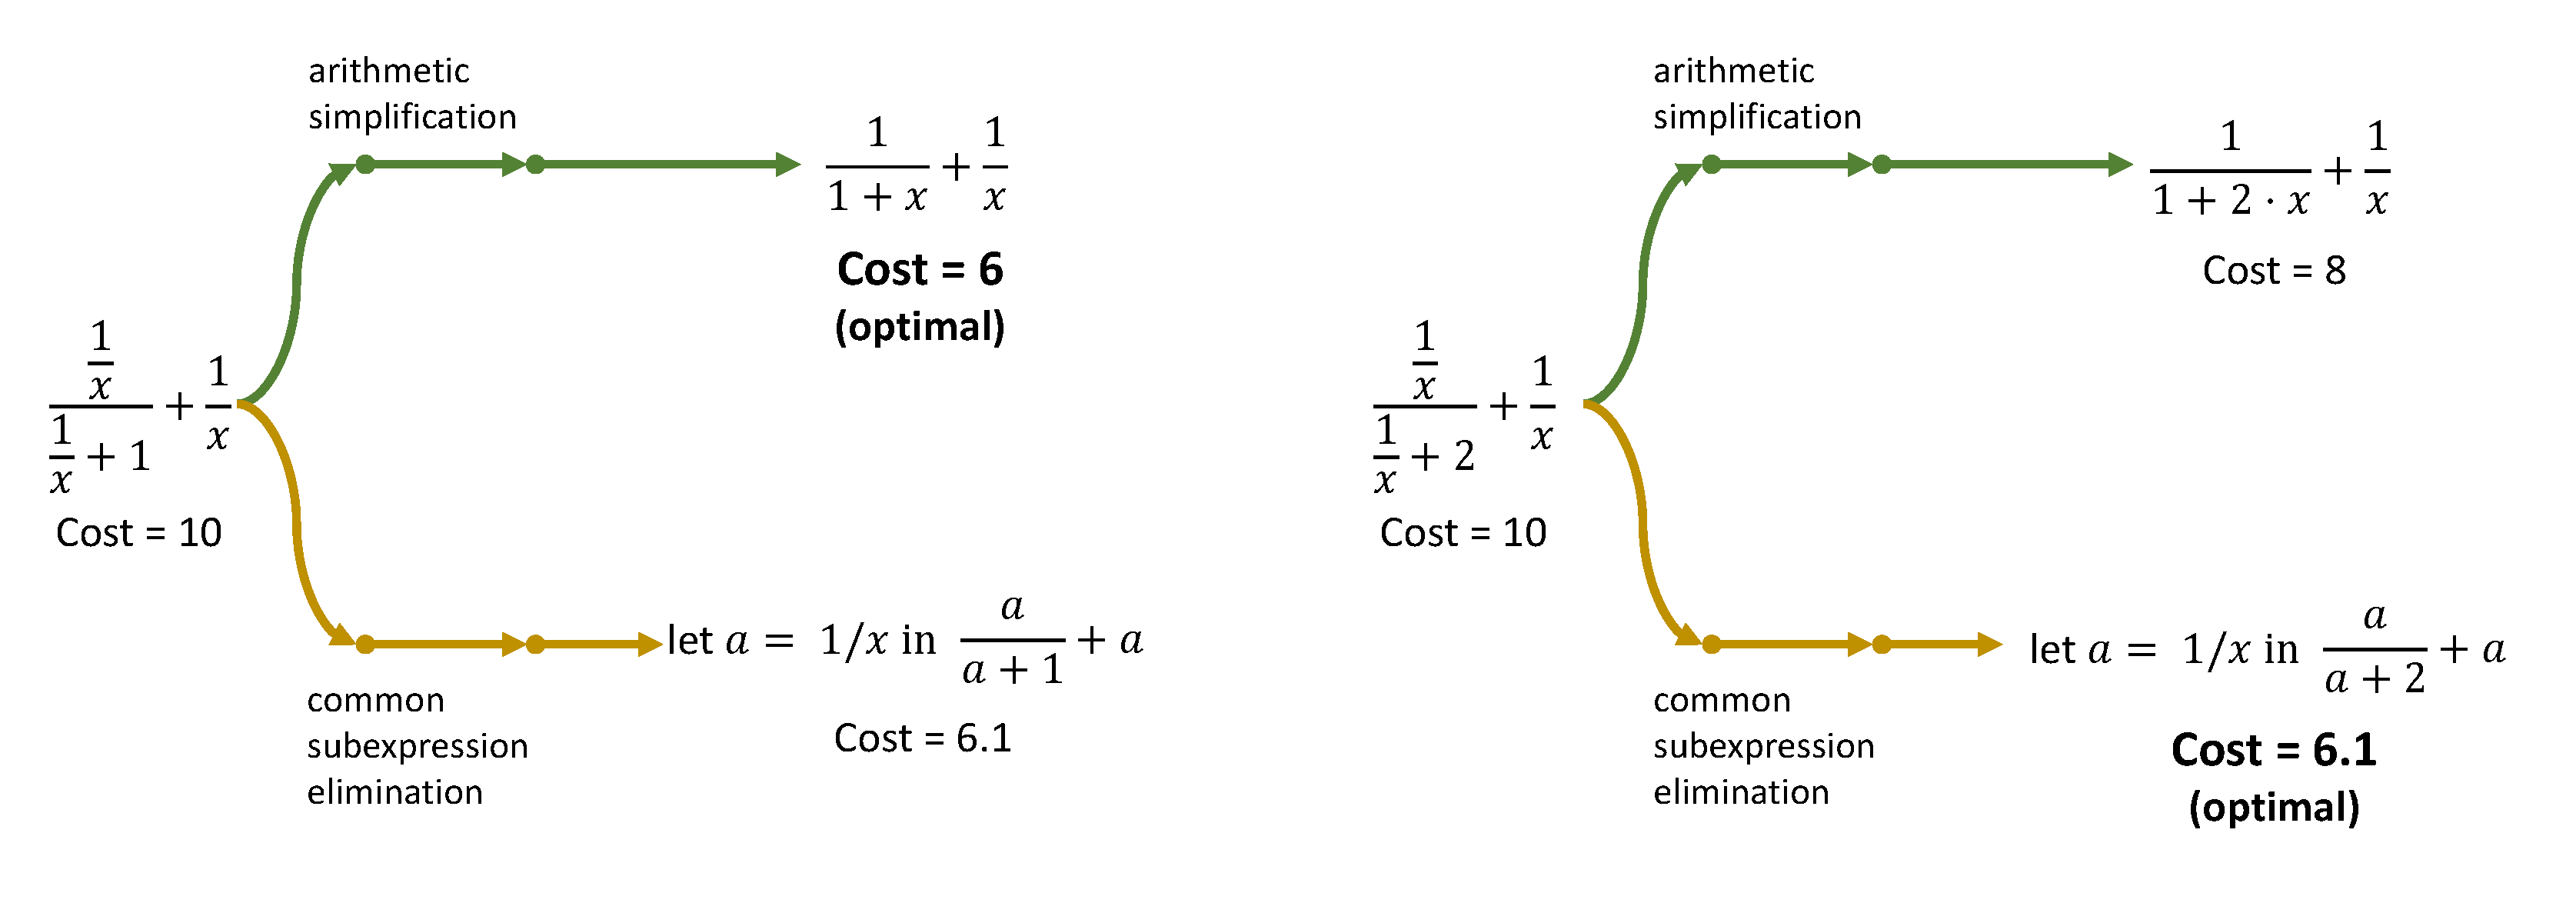
\includegraphics[width=1.0\textwidth]{tricky-expression.pdf}
  \caption{Example of tricky optimisation task. Two expressions are similar but the optimal rewrite strategies are different.}
  \label{trickey-example}
\end{figure*}


% We don't have any huge expressions in the benchmark expression set yet. So this statement is not appropriate for this submission.
The task of rewriting expressions is distinct from traditional RL benchmarks in two main ways. First, the number of actions possible in a certain state might be of the order of 10,000, much higher than the number of admissible moves in the game of Go \citep{Silver2016, silver2017mastering}, which is at most 361 in the 19$\times$19 version. This means that our state space is more complex. For example, an expansion of the Go search tree with horizon 20 has about $10^{51}$ states while our MDP has $10^{80}$ even for relatively easy examples. 

\paragraph{Hard and Easy Aspects of Rewriting} 
There are two main ways in which the task of rewriting expressions is \emph{more challenging} than typical RL benchmarks. First, the allowed set of actions not only changes from state to state, but grows with the size of the expression. This makes exploration hard. Second, the states of the MDP, which correspond to the expressions being rewritten, are represented as graphs, whose size and topology varies as optimisation progresses. This is unlike traditional deep Reinforcement Learning \citep{mnih2013playing}, which learns either from pixels or from data of fixed shape. While the rewriting task has many features that make it difficult, \emph{it is also easier} than many traditional RL tasks for three reasons. First, MDP transitions are completely deterministic. Second, the task has a large degree of locality in the sense that the performance of a program can often be substantially improved by optimising its parts separately. Third, we can generate state transitions in any order convenient to us, as opposed to the traditional RL setting, where we are constrained by the order imposed by the environment. Overall, we have a problem similar to traditional planning, but which requires us to generalise well in order to obtain competitive solutions. To do this,  Knossos uses a custom RL algorithm, based on $A^\star$ search supported by value function learned with a graph neural networks (Algorithm \ref{lst:knossos}). We describe how to obtain the heuristic in Section \ref{sec-graph-nn}, and the search algorithm in Section \ref{sec-a-star}.


\begin{algorithm*}
\caption{Knossos}
\begin{algorithmic}
    \Function{Train}{$E_{\text{train}}, H, M$}
           \State $\text{{\bf Input:} } E_{\text{train}}$: Set of expressions to train
           \State $\hphantom{\text{{\bf Input:} } E}\mathllap{H}$: Maximum depth of the search
           \State $\hphantom{\text{{\bf Input:} } E}\mathllap{M}$: Number of epochs
        \State Initialize a value function $\hat{V}$

        \For {$M$ iterations }
            \For {$e \in E_{\text{train}}$}
                \State $S, \Vtarget \leftarrow A^\star(e, \hat{V}, H)$
                \Comment{Optimize $e$ and store the learned values $\Vtarget$}
                \State $\hat{V} \leftarrow \textsc{Fit}(S, \Vtarget, \hat{V})$
                \Comment{Fit the value function - see Section \ref{sec-graph-nn}}
            \EndFor
        \EndFor
    \EndFunction
    \\
    \Function{Optimize}{$e, \hat{V}, H$}
    	   \State $\text{{\bf Input:} } e$: Expression to optimize
    	   \State $\hphantom{\text{{\bf Input:} } e}\mathllap{\hat{V}}$: Learned value function
    	   \State $\hphantom{\text{{\bf Input:} } e}\mathllap{H}$: Maximum depth of the search
        \State $S, \_ \leftarrow A^\star(e, \hat{V}, H)$
        \Comment{Optimize $e$}
        \State \Return $\argmin_{s \in S} c(s)$
        \Comment{Return the best expression found during the process}
    \EndFunction
\end{algorithmic}
\label{lst:knossos}
\end{algorithm*}

\subsection{Searching the space of rewrites with $A^\star$}
\label{sec-a-star}
\begin{algorithm*}
\caption{Deep $A^\star$ search}
\begin{algorithmic}
    \Function{$A^\star$}{$e_0, H, \hat{V}, T$}
    \State $\text{{\bf Input:} } e_0$: Expression to optimize
    \State $\hphantom{\text{{\bf Input:} } e_0}\mathllap{H}$: Maximum depth (time budget) of the search
    \State $\hphantom{\text{{\bf Input:} } e_0}\mathllap{\hat{V}}$: Learned value function, maps (expression, time left) to predicted best cost
    \State $\hphantom{\text{{\bf Input:} } e_0}\mathllap{T}$: Transition function, maps (expression, action) to rewritten expression
    %\State $f(s) \leftarrow t_s\cdot\hat{V}(s) + \sum_{i=0}^{H-t_s-1} R(s_i, s_{i+1})$ %this isn't actuall evalauted here
    \State $s_0 \leftarrow (e_0,H)$    
            \Comment{State is $(e,t)$, where $t$ represents the step budget left for the expression $e$.}
    \State push($\open{}, s_0, \infty$)
    				\Comment{Push state $s_0$ on (probabilistic) priority queue $\open{}$ with highest priority, i.e. first to pop}
    \State $\closed{} \leftarrow \{s_0\}$
            \Comment{$\closed{}$ is a list storing all states visited}
    \While {{\bf not} \textsc{term\_condition}() and $\open{}$ is not empty}
        \State $s = (e,t) \leftarrow pop(\open{})$             \Comment{Take next most promising state $s = (e,t)$ from priority queue}
        \ForAll {$a \in A(e)$}                                 \Comment{For all actions $a$ valid at expression $e$}
            \State $s' = (e',t') \leftarrow (T(e, a), t-1)$ 
                                  			\Comment{Apply action $a$ to state $s$, giving new expression $e'$ and time $t'$}
			\def\seen{\text{seen}}
		   \State{$\seen = \{\tau\mid (e',\tau) \in C\}$} \Comment{Remaining time for matches of $e'$ in $C$, or empty set $\emptyset$ if no match}
            \If {$\seen = \emptyset$ \textbf{or} $\min(\seen) < t'$}
                \If {$t' > 0$} \Comment{Time remaining is nonzero, there are states to be explored}
                    \State push($\open{}, s', f(s')$)
        \Comment{Priority function $f$ is the heuristic defined in equation \ref{eq-heuristic}.}
                \EndIf
                        \State $\closed{} \leftarrow \closed{} \cup \{s'\}$
            \EndIf
        \EndFor
    \EndWhile
    \ForAll {$s \in \closed{}$}
        \State $\Vtarget(s) \leftarrow \max \{ \left(c(e_s) - c(e')\right) \mid (e',t') \in \closed{} \textbf{ and } t' \leq t_s \} $ %  \sum^{t(s')}_{k'=t_s} r_{k'}
		\LineComment{Empirical estimate of maximum cost reduction achievable from $s$}
    \EndFor
    \State \Return $\closed{}$, $\Vtarget$
    \EndFunction
\end{algorithmic}
\label{lst:astar}
\end{algorithm*}

We use the $A^\star$ algorithm \citep{hart1968formal} both to train the compiler and to deploy it. $A^\star$ maintains two priority queues. One queue ($O$) stores the frontier, i.e.\ states from which transitions have not been explored yet. The other one ($C$) stores the states visited so far and is used to avoid exploring the same path twice. The states are explored in the order induced by the $A^\star$ heuristic, which in our case corresponds to the learned value function $\hat{V}$, obtained from previous iterations. In particular, node priority is set as follows:
% (from Kamil) The description below looks a bit too details for an AI audience given how popular A* is. I have made it more concise.
% Feel free to restore this if you disagree
Each iteration of $A^\star$ is as follows (Algorithm \ref{lst:astar}). First, an agent picks a node which has the highest priority. Then, it generates all the child nodes of the node. For each generated child node, it queries the closed list to check if we already visited that state. If the child state $n$ is not visited for any time budget $t$ ($(e_n, t) \notin \closed{}$), or visited only with less remaining time ($t(n) > t$), then it is stored in the open list. We  repeat this procedure until some termination condition is satisfied.
%$A^\star$ picks a node which has the highest priority $f$ in the open list. 
%We set the priority of a node $n$ to be the estimated total cost reduction from the initial expression. % the cost reduction achieved at $n$ plus the estimated possible cost reduction from $n$:
\begin{gather}
\label{eq-heuristic}
    f(s) = f(\underbrace{(e_s,t_s)}_s) =  \hat{V}(s) + \underbrace{\textstyle \sum_{i=0}^{H-t_s-1} R(s_i, s_{i+1})}_{c(s_0) - c(s)}.
\end{gather}

Here, $\hat{V}(s)$ is the estimated future cost reduction obtained from state $s$ within $t$ remaining time-steps. The quantity $c(s_0) - c(s)$ corresponds to the cost reduction that has already been achieved by time $t$, measured against the cost of the initial expression. Thus, $f(s)$ is an estimate of the maximum possible cost improvement from a trajectory passing through state $s$ at time $t$.

% (from Kamil: that message was merged into the begiinning of Section 3)
%While typical model-free reinforcement learning algorithms select next state to explore subject to a constraint that it has to be a neighbor of the state it jused explored, $A^\star$ has no such constraint.  Such constraint is required for typical reinforcement learning domains where an agent is not allowed to change the state of the environment or the cost of copying states is huge or impossible (e.g. robotics task). However, for a graph search problem where such constraints doesn't exist, $A^\star$ is a powerful algorithm as it has less constraint on which state to explore next.

After the search, we compute the empirical estimate of the maximum cost reduction achievable ($\Vtarget(s)$) for each visited state.  The estimated value of $s$ with $t_s$ timesteps is the maximum cost reduction found from $s$ within $t_s$ steps. $\textsc{distance}(s, s')$ in Algorithm \ref{lst:astar} is the number of steps required to reach $s'$ from $s$. The algorithm stops after the value function was evaluated a set number of times. In the code this is represented with the function $\textsc{term-condition}$.

$A^\star$ is well-suited for the rewriting task because it exploits its characteristic features. In particular, it exploits determinism by assuming that a cost reduction achievable once can always be achieved again. It exploits the availability of reset by considering nodes in the order defined by the heuristic function. It exploits locality by preferring re-writes that need a small number of rule applications. Before deciding on $A^\star$ , we also performed experiments with Monte Carlo Tree Search (MCTS). MCTS does not make use of reset and had worse empirical performance (see \ref{ablation-mcts} for details). 

\subsection{Learning Value Functions with Graph Neural Networks}
\label{sec-graph-nn}
States in the Knossos MDP correspond to computation graphs. In order to apply deep RL to these graphs, we need to be able to construct differentiable embeddings of them. To do this, we employ Graph Neural Networks based on Gated Recurrent Units \citep{DBLP:journals/corr/LiTBZ15}. During the forward pass, the GNN begins with an initial embedding of the graph nodes. It then iteratively applies a diffusion process to the graph. At each step, the obtained representation is fed into a gated recurrent unit (GRU). The process implicitly encodes the edge structure of the graph in the obtained representation.

\paragraph{Graph representation}
We represent a Knossos expression as a graph. The graph nodes correspond to subexpressions (see Fig.~\ref{sample-state}). The graph edges are of two kinds. The first kind of edges connects the nodes with their parents. In addition, we use another kind of edges, which is used to explicitly provide the information that two subexpressions are identical. See Table \ref{tab:edge-types} for a list of all edge types. Edges can be directed or undirected, with the directed edges going in opposite ways considered different.

\begin{figure*}[t]
\begin{subfigure}[b]{.5\textwidth}
    \centering
    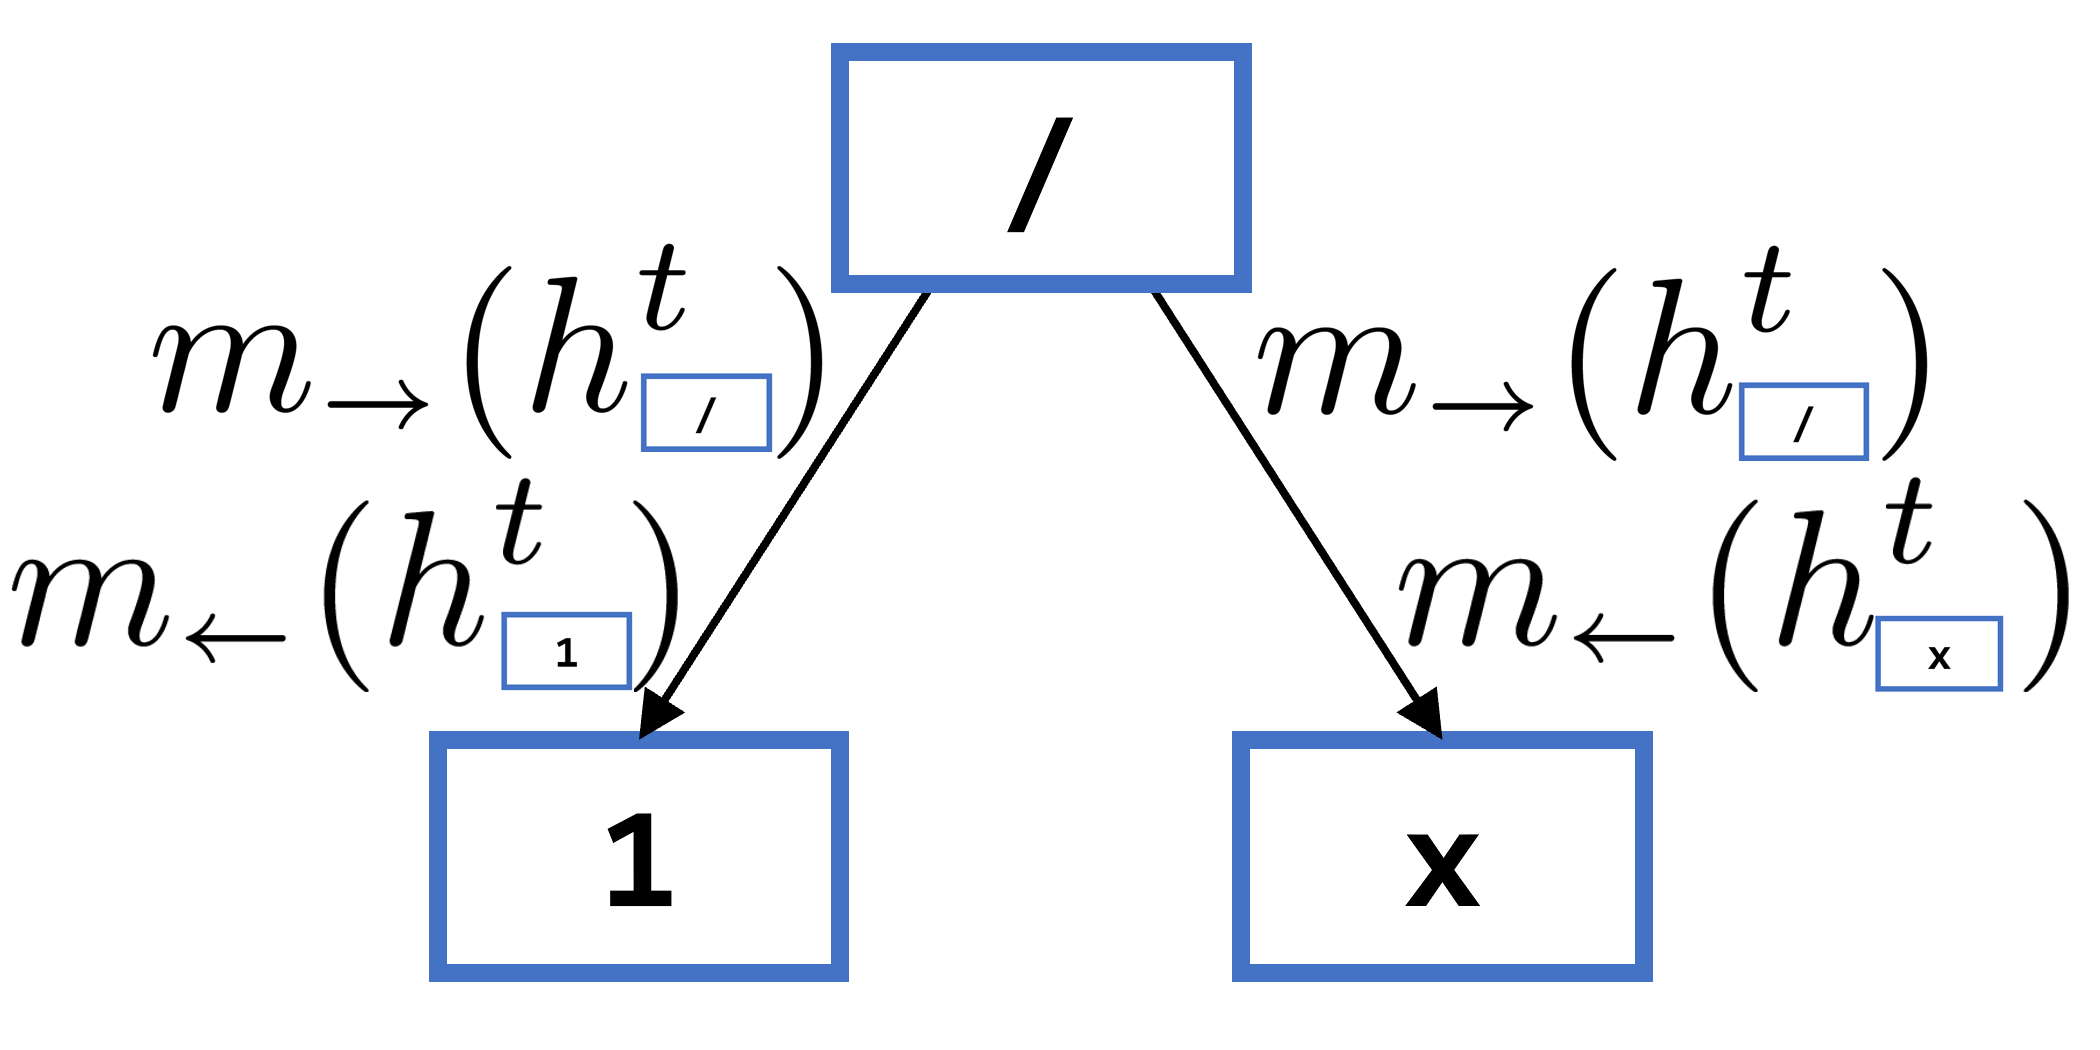
\includegraphics[width=5cm]{gnn_plot_larger}
    \caption{Message passing on the expression graph.}
    \label{value-function}
\end{subfigure}~\begin{subfigure}[b]{.5\textwidth}
    
    {\small\centering
    \begin{tabular}{p{1.8cm}p{1.8cm}}
    \toprule
    \bf{Edge type} & \bf{Directionality} \\ \midrule
    first child & directed \\
    second child & directed \\
    third child & directed \\
    tuple child & directed \\
    is-identical & undirected \\ \bottomrule
    \end{tabular}
    \caption{List of edge types}
    \label{tab:edge-types}
    }
\end{subfigure}
\caption{Graph neural network}
\end{figure*}


\paragraph{Graph neural network}
To compute the value function for an expression $e$ and time budget $t$, we start from computing the initial node embedding $h_v^{0}\in \mathbb{R}^d$ for all node $v\in N(e)$, where $N(e)$ is the set of vertices in expression $e$. The initial node embedding consists of a one-hot encoding of the node type (constant, variable, etc) followed by zero padding.

This embedding is then fed into the following recurrent computation (see Fig. \ref{value-function}):
\begin{equation}
\label{eq-gnn-recurrence}
        \textstyle h_v^{t+1} = f\left(h_v^{t}, \Oplus_{
\substack{v'\in A_{p}(v), \\ p \in P}
}m_p\left(h_{v'}^{t}\right)\right)\quad (t=0,\ldots, T-1),
\end{equation}
where $p\in P$ indexes different edge types, $A_p(v)$ is the set of neighbors of node $v$ with respect to the $p$th edge type. We choose the message function $m_p$ to be a single dense layer for each edge type $p$ and the aggregation operator $\oplus$ as the sum of all incoming messages. We use the GRU cell \citep{cho2014learning} as the recurrent unit $f$.
%
The final node embedding $h_v^{T}$ is computed by unrolling equation \ref{eq-gnn-recurrence} for $T$ time steps.

Finally the value of expression $e$ is computed by taking a weighted sum of the final node embedding $h_v^{T}$ and passing through a dense layer as follows:

\begin{equation}
    \boldsymbol{V}(e) = \textstyle O\left(\sum_{v\in N(e)}\sigma\left(g(h_v^{T}, h_v^{0})\right)\cdot r(h_v^{T})\right)
\end{equation}
where $g:\mathbb{R}^{2d}\rightarrow\mathbb{R}^d$, $r:\mathbb{R}^d\rightarrow\mathbb{R}^d$, $O:\mathbb{R}^d\rightarrow\mathbb{R}^H$ are all one-layer dense networks, $\sigma$ denotes the sigmoid function, and $\boldsymbol{V}(e) = [V((e,0)), V((e,1)),\ldots,V((e, H-1))]^\top\in\mathbb{R}^H$.

% Our graph embedding is a sum over node embeddings. Intuition is that the amount of future improvement can be approximated by the sum of its local improvements.

% We are not collecting roll-outs. What's the best way to explain this?
We train the above GNN to approximate the optimal value function $V^\star$. Let $\bar{V}(s)=\boldsymbol{V}(e_s)[t_s]$ the value function $\boldsymbol{V}$ computed for expression $e_s$ and time budget $t_s$.
%
% Having obtained a roll-out $\tau_\pi = \left( s_1, a_1, r_1, s_2, a_2, r_2, \dots s_H, r_H \right )$ from the policy $\pi_V$, we update the estimate of the value function. % We do not have a rollout. How Vtarget is computed is explained in A* instead.
To track an approximate lower bound of the optimal value function $V^\star$,
we minimize the loss $l(\bar{V}(s) - \Vtarget(s) / t_s)$. The target value $\Vtarget(s)$ is defined in Algorithm \ref{lst:astar} and corresponds to the best cost improvement obtained with the current policy in $t_s$ steps.
Normalization by $t_s$ is introduced to ease optimisation by ensuring that target values for all outputs of $\boldsymbol{V}$ are in a similar magnitude. Thus the value function estimate $\hat{V}(s)$ can be obtained from per-step value estimate $\bar{V}(s)$ as $\hat{V}(s)=t_s\cdot \bar{V}(s)$.
For the loss function $l$ we use the Huber loss. Details about the optimiser used to minimize the loss $l$ are given in  \ref{sec:exp-setup}. In the pseudocode in Algorithm \ref{lst:knossos}, this optimisation is represented with the function \textsc{fit}.

% so that it is robust to outliers.

% (Kamil: since we don't have recursion, we should proably skip this)
We stress that our GNN works seamlessly with programs which include recursive function calls. Naively, it may seem that allowing recursion in Knossos expressions would lead to an infinite expansion, making GNN inference impossible. Fortunately, this is not the case.  Knossos represents calls to the same recursive function by graph nodes with shared labels, rewriting the abstract syntax tree of a program rather than its stack trace. In other words, using recursion does not lead to explosion in the size of the computation graph for the same reason that recursive programs do not take an infinite number of lines of code to write. % We don't have recursive function in a benchmark expression set.


\subsection{Curriculum Learning}
 \label{sec-curriculum}
Due to the scale of the search problem in Knossos, it is difficult to obtain a good agent by immediately training on the hardest-to-optimize programs. In order to address this problem, we follow a curriculum \citep{elman1993learning, bengio2009curriculum} when training the agent. In each training epoch, we associate a \emph{success rate} $\SuccessRate$ with each expression. The success rate $\SuccessRate$ counts, the proportion of rollouts which reached the current best-known value for each expression. During training, we only consider expressions with success rate $p_L < \SuccessRate < p_H$, where $p_L$ and $p_H$ are hyper-parameters. By excluding expressions which are either trivial or intractable from training, we allow the agent to make faster progress. Our results in section \ref{sec-benchmarks} show that this curriculum is very effective. 
% 
% (TODO: more detail).

%In order to ensure that the dataset is balanced, we 


\section{Related Work}
\label{sec-related-work}
Knossos builds on a long tradition of compiler technology. Similarly to traditional compilers \citep{santosProgramTransformationGlasgow1992, lattnerLLVMCompilationFramework2004} and the more recent deep learning compilers such as  Myia \citep{merrienboerAutomaticDifferentiationML2018}, DLVM \citep{weiDLVMModernCompiler2018},  ISAM \citep{sotoudehISAMapperCompute2019} and GLOW \citep{rotemGlowGraphLowering2018}, Knossos uses an intermediate representation to optimize programs. However, while these approaches rely on layers of hand-coded optimisation heuristics, Knossos \emph{learns} the algorithm used to optimize its programs.

In this respect, Knossos is a spiritual successor of benchmark-driven hardware-agnostic optimisation approaches in computational linear algebra \citep{paduaAutomaticallyTunedLinear2011} and signal processing \citep{frigoFFTWAdaptiveSoftware1998}. However, unlike these approaches, Knossos is a fully-fledged compiler, and can optimize arbitrary programs. Moreover, thanks to its Reinforcement Learning-driven optimizer, Knossos has an advantage over existing approaches that attempt to learn how to optimize arbitrary code. For example, \citet{bunelLearningSuperoptimizePrograms2017} learns parameters of a code optimizer with a hard-coded hierarchy. REGAL \citep{paliwalREGALTransferLearning2019} only learns the hyper-parameters for a fixed genetic algorithm that preforms the actual optimisation.  The TVM compiler \citep{chenTVMAutomatedEndtoEnd2018} learns a cost model over programs, but uses simple simulated annealing to perform the optimisation. Similarly, \citet{chenLearningOptimizeTensor2018} handles only index summation expressions and again relies on simulated annealing. LIFT \citep{lift-paper} defines an intermediate language suited for expressing numerical computation, but focuses on providing the right set of rewrite rules rather than on the program optimisation process itself. In Section \ref{sec-benchmarks}, we demonstrate that the RL optimizer used by Knossos outperforms this approach by a large margin.

Knossos is also related to JAX \citep{jax}, which performs just-in-time compilation of Python code using the XLA backend \citep{xlaauthorsTensorFlowXLAAccelerated2016}. Knossos differs from JAX in two ways. First, it uses efficient RL code optimisation, which is architecture-agnostic. In fact, since Knossos generates \Cpp code, it supports a much broader variety of target architectures. Also, unlike JAX, it makes use of the benefits of a statically typed languages. In terms of scope, Knossos is also similar to Zygote for Julia \citep{innes2019zygote}. However, unlike these compilers, Knossos makes use of an RL-driven code optimizer.

Since Knossos provides first class support for automatic differentiation, it is also related to established deep learning frameworks \citep{maclaurinAutogradEffortlessGradients2015, abadiTensorFlowSystemLargeScale2016, paszkeAutomaticDifferentiationPyTorch2017a}. However, unlike Knossos, these frameworks do not learn how to optimize code, instead relying on manually-prepared back-ends. Moreover, using them either requires meta-programming, where the user  has to use a high-level language to specify the desired computation graph using constructions external to the language \citep{abadiTensorFlowSystemLargeScale2016}, or is constrained to a restricted subset of the language \citep{paszkeAutomaticDifferentiationPyTorch2017a}. In contrast, the Knossos language can be used directly, without manually specifying  computation graph constructs or restricting oneself to an allowed subset of the language. 

In parallel, the idea of automated rewriting to achieve a given objective was explored in the context of automated theorem provers. This is conceptually related to our approach since finding an equivalence between formulae is the same as finding a proof that they are equal. However, recent work in this space has substantial differences in scope. In particular, state-of-the-art work that searches for refutational proofs in first-order logic \citep{zomboriFindingLongerProofs2019, kaliszykReinforcementLearningTheorem2018} uses hard-coded features and cannot learn any new ones. Also, the optimal objective is very different. While a mathematical proof is only correct when completely reduced to a tautology, we are satisfied with simplifying an expression by a certain margin, not necessarily in the most optimal way possible. 

For the Reinforcement Learning part, our algorithm differs from standard techniques in that it has a much larger action space and a state space that consists of graphs, which makes the application of traditional RL algorithms like DQN \citep{mnih2013playing}, A2C \citep{mnih2016asynchronous} and PPO \citep{schulman2017proximal} ineffective. AlphaGo \citep{Silver2016, silver2017mastering}, which also performs a search over a large state space, but differs from Knossos in that it learns for pixel observations and uses an action space of bounded size. Reinforcement Learning has also been applied to expression rewriting and scheduling problems \citep{chen-rewrite-schedule}. However, since this approach used actor-critic RL that does not exploit reset, it less well-suited for compilation tasks as described in Section \ref{sec-training}.


\section{Benchmarks}
\label{sec-benchmarks}


We evaluated Knossos in three settings. First, to understand how close and reliably we can achieve the best optimisation, we applied Knossos to a manually curated set of arithmetic expressions, where we know the best available sequence of rewrites. Second, we applied Knossos to a set of linear algebraic operations, which are representative of typical workloads in numerical computing. 
Third, we implemented a Gaussian Mixture Model (GMM) to asses how the code optimizer scales to more realistic tasks, including differentiation. 
Fourth,
in order to reflect common modern use-cases, we evaluated Knossos on a computer vision task that uses a convolutional neural network.  Since Knossos is as an alternative to traditional compilers,
we compare it to a hand-written rule-based transpiler of the Knossos IL, which we call \texttt{ksc}. Both Knossos and \texttt{ksc} output \Cpp, which is compiled to binary using \texttt{gcc} \emph{with optimisation enabled}, ensuring a fair comparison. We describe the results below. 



\begin{figure*}[t!]
	\centering
  	\begin{subfigure}[t]{0.45\textwidth}
  		\centering
	    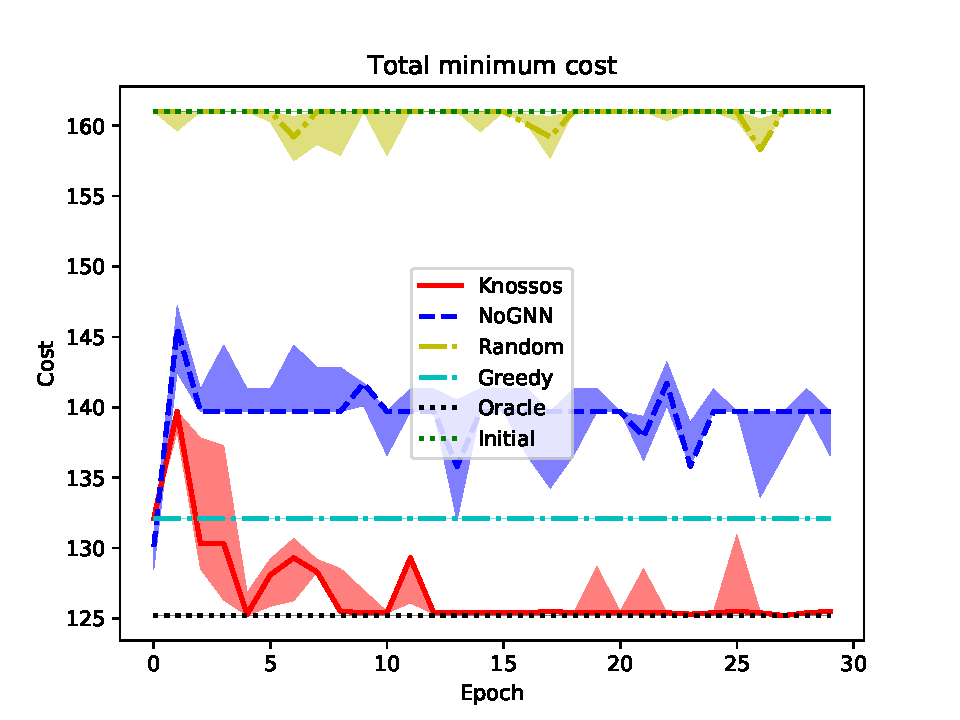
\includegraphics[width=\textwidth]{generalization.pdf}
	    \caption{Generalisation to Unseen Data}
	    \label{generalization}
	\end{subfigure}%
  	\begin{subfigure}[t]{0.45\textwidth}
  		\centering
	    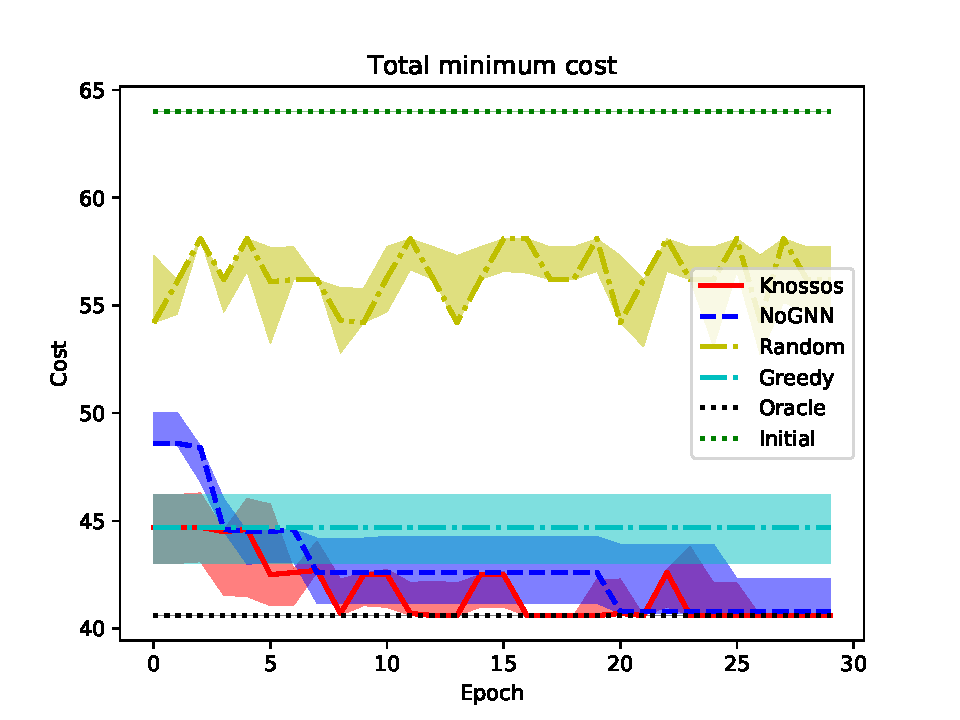
\includegraphics[width=\textwidth]{combined.pdf}
	    \caption{Bootstrap Mode}
	    \label{combined}
	\end{subfigure}
    % \hspace{-2.5cm}
    \caption{Performance of Knossos on a set of arithmetic expressions. Horizontal axis shows epochs, vertical axis shows cost. Shaded area spans the 20\% and 80\% percentile over 10 repetitions.}
    \label{benchmark-arithmetic}
\end{figure*}

\paragraph{Generalisation to Unseen Data}
While arithmetic expressions are simple, optimising them is not always a simple task.
Figure \ref{trickey-example} shows an example of two similar arithmetic expressions.
Although they look very similar, they require different optimisation strategy to reach to the optimal form. The left expression gets to optimal by an arithmetic simplification ($\times x$ to a denominator and a numerator) but the right expression gets to optimal by a common subexpression elimination. It is difficult for a rule-based compiler to distinguish the two and optimise such similar expressions using different strategies.
To test Knossos on arithmetic expressions, we used a training set of 36 arithmetic expressions and a test set of 12 different ones. The details of the experimental setup are given in \ref{sec:exp-setup}. 
In this setting, we pick 6 expressions randomly from a training set to train in each epoch. We ran training for 30 epochs and running 10 repetitions for each experiment with different random seeds.
%
Search depth was limited to 10 and the termination condition in $A^\star$ was set to 5000 evaluations of the value function. See \ref{sec:exp-setup} for the full details including network parameters. We show the results in Figure \ref{generalization}. It can be seen from the figure that Knossos achieved the oracle cost for all expressions. We also performed an ablation, comparing Knossos to $A^\star$ algorithm (shown as NoGNN) that does not perform the GNN recurrence in equation \ref{eq-gnn-recurrence}. As a baseline, we compared to greedy best-first search, which picks a next state to explore greedily without using the value function $f(s) := c(s_0) - c(s)$. We also show a comparison to random search and the initial cost of the expression, before any optimisation.

% (metnion of MCTS was moved to section 3) We also evaluated the performance of Knossos using Monte Carlo Tree Search as a search engine. See appendix for the comparison of the performance of search engines. (TODO). 

%The yellow dash dotted line at the bottom shows the total minimum cost achievable and the blue dash dotted line at the top shows the total cost of the initial expressions.

%Figure \ref{benchmark-arithmetic} shows the performance of the Knossos code optimizer on a set of arithmetic expressions as a function of training epochs. Horizontal axis shows the number of training epochs. Vertical axis shows the minimum cost found by an agent trained for that number of epochs, summed over the test set. 

% Simplify and Binding tasks are too easy to compare the performance of the search algorithms but we show the performance on them for record.
% Double check all the hyperparameters for the experiment. 
% We do not evaluate the value of $V(s)$ for the same expressions twice in the epoch as we cache the value for expressions visited. % We never visit the same expression twice in A*.

% Figure \ref{benchmark-arithmetic} shows the performance of the Knossos code optimizer on a set of arithmetic expressions as a function of training epochs. The top plot shows the attained cost reduction for each expression, while the bottom plot shows the success rate, i.e. the percentage of rewrites that achieve the best possible performance. Shaded areas in the plots measure the spread across outcomes, measured as the difference between the best and worst run after performing TODO independent runs. The plot indicates that all expressions successfully match the optimal rewrite with probability at least 80\% after 60 training epochs. Moreover, the results match the basic intuition about how hard it is to solve each expression. For example, the expression where the possible cost reduction is the largest takes the longest to reliably simplify.


\paragraph{Bootstrap Mode}
Similarly to a traditional compiler, where we are given a concrete program to optimize, the expressions used to evaluate Knossos in this benchmark were the same ones that we used used during training. Even in this setup, Knossos still generalises, but it does it across sub-expressions of the expressions in the training set. 
We tested that on 8 expressions, training for 30 epochs. Other experimental setup is the same as Arithmetic Expressions.
Figure \ref{generalization} shows the comparison of the minimum cost achieved by each agent.
It can be seen from the figure that Knossos achieved the best possible cost for all expressions.

\paragraph{Linear Algebra Primitives}
Numerical linear algebra is fundamental to most calculations in scientific computing and machine learning. Primitives such as vector multiplication, plane rotation, matrix multiplications and similar primitives often represent the most time-consuming part of the given computation. To evaluate the performance of Knossos on in this setting, we trained on a set of 11 such linear algebra primitives and evaluated on General Matrix Multiplication (GEMM). We trained for 5 epochs, each of which included optimisation of cost of 6 primitives. Search depth was limited to 30 and the termination condition in $A^\star$ was set to 5000 evaluations of the value function. Figure \ref{benchmark-blas} shows the cost of GEMM. The plot shows results for 10 independent runs of the Knossos code optimizer on the same input source file.
We used an augmented set of training rules, which included vector operations (see Table \ref{tbl:extended_rules} in Appendix). Because of the complexity of the task, we split the search into two phases of 15 steps each. The training phases differ in the set of allowed rules. In the first phase, we only allow rules that result in large changes to the cost (Table \ref{tbl:extended_rules}). In the second phase, we allow all rules.
The shaded area represents one standard deviation across the runs of Knossos. Results show that Knossos produced code of lower cost than the output of the traditional \texttt{ksc} compiler according to our cost model. We also performed a benchmark using wall clock time, shown in Fig.~\ref{benchmark-time-blas}, again showing an improvement. In addition, we performed a qualitative evaluation of the output in Fig.~\ref{gemm-qualit}.  In the program obtained by \texttt{ksc} (middle listing), three temporary variables \texttt{mat\_x}, \texttt{mat\_x\_6}, and \texttt{mat\_y} corresponding to the result of $A\cdot B$, $\alpha\cdot\texttt{mat\_x}$, and $\beta\cdot C$, respectively, are created. In the output of Knossos (bottom listing), all the temporary variables are gone. Hence, Knossos has discovered a form of loop fusion -- the type of optimisation that previously had to be built into a compiler by a laborious manual process.


  
%The figure is already doing that.
%\todo{Sketch of what the codes are doing.}


%\begin{figure*}[t!]
%        \centering
%        \begin{subfigure}[t]{0.31\textwidth}
%                \centering
%            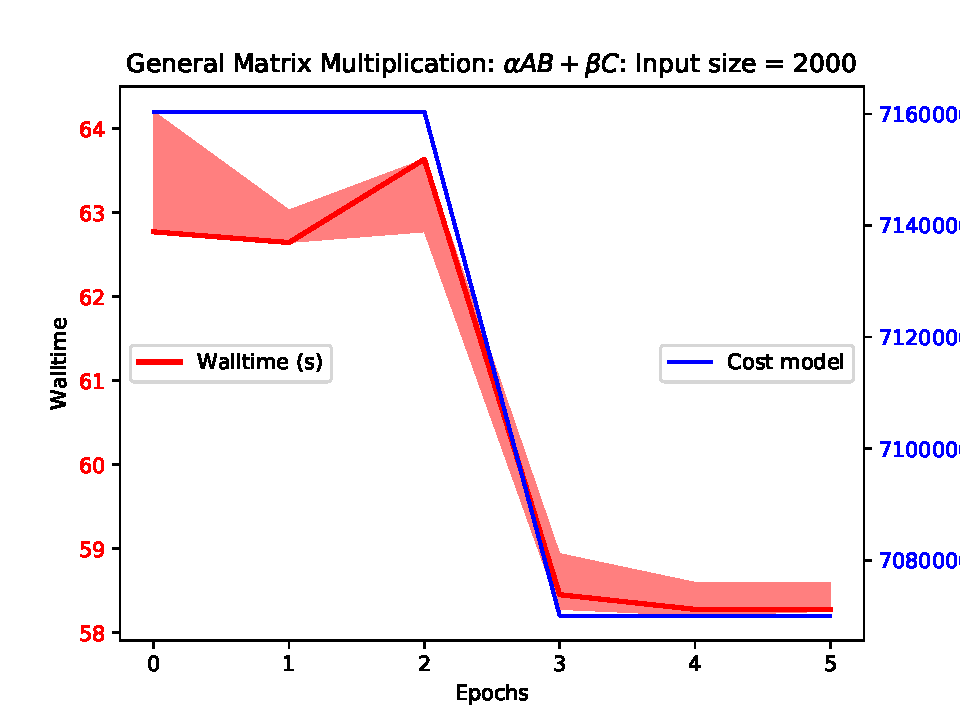
\includegraphics[width=\textwidth]{blas-epochs-walltime2000.pdf}
%            \caption{Basic Linear Algebra}
%            \label{benchmark-blas}
%        \end{subfigure}
%        \begin{subfigure}[t]{0.31\textwidth}
%                \centering
%            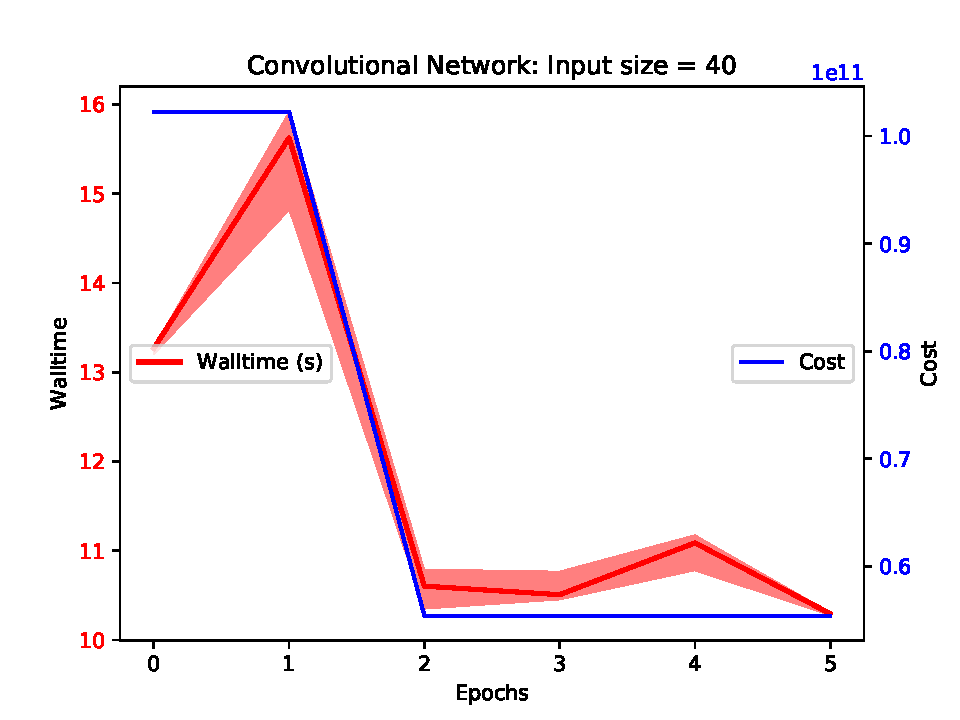
\includegraphics[width=\textwidth]{cnn-epochs-walltime40.pdf}
%            \caption{Convolutional Neural Network}
%            \label{benchmark-cnn}
%        \end{subfigure}
%    % \hspace{-2.5cm}
%    \caption{Performance of Knossos on basic linear algebra and convolutional network. Shaded area indicates one standard deviation.}
%    \label{benchmark-ml}
%\end{figure*}

%\begin{figure*}[t!]
%        \centering
%        \begin{subfigure}[t]{0.31\textwidth}
%                \centering
%            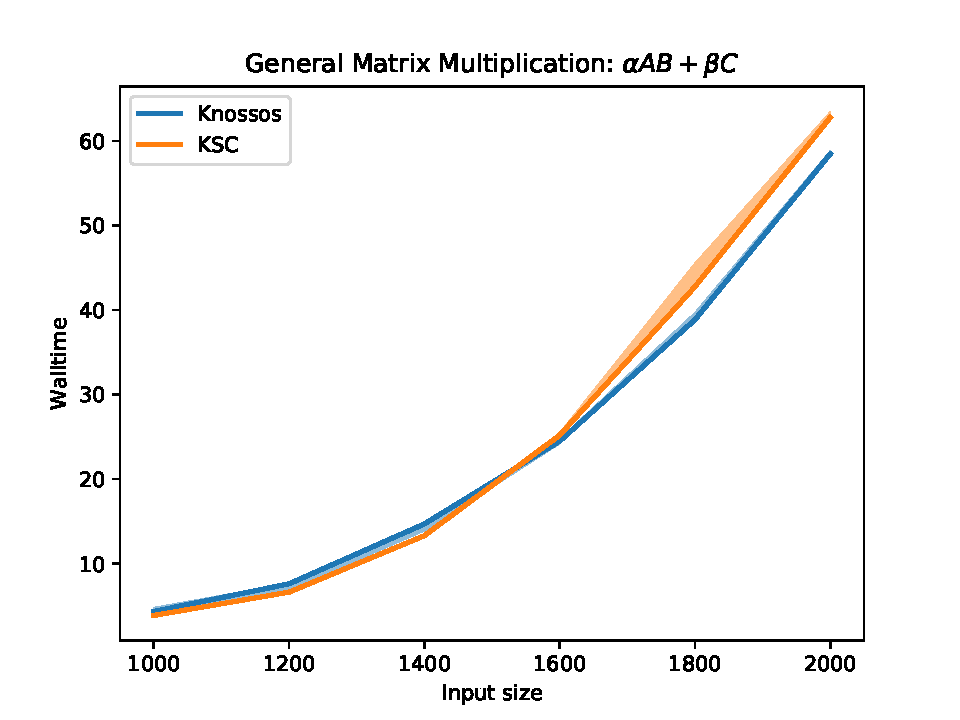
\includegraphics[width=\textwidth]{blas-inputsize-walltime.pdf}
%            \caption{Basic Linear Algebra}
%            \label{benchmark-time-blas}
%        \end{subfigure}%
%        \begin{subfigure}[t]{0.31\textwidth}
%                \centering
%            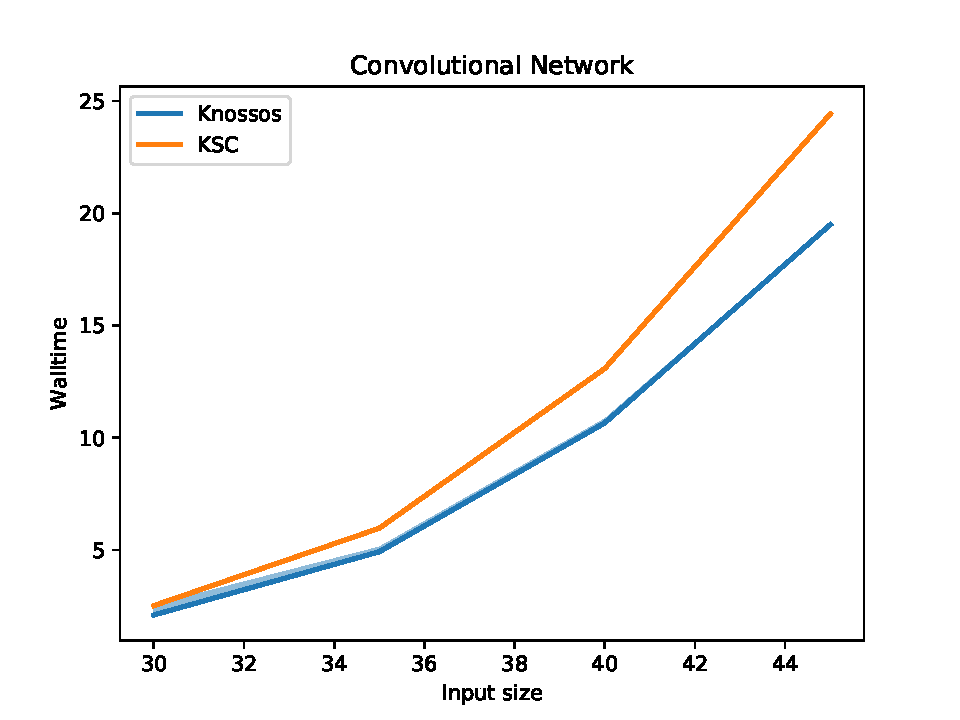
\includegraphics[width=\textwidth]{cnn-inputsize-walltime.pdf}
%            \caption{Convolutional Neural Network -- wall time comparison with \texttt{ksc}.}
%            \label{benchmark-time-cnn}
%    \end{subfigure}
%    % \hspace{-2.5cm}
%    \caption{Comparison of wall time. Shaded area indicates one standard deviation.}
%    \label{benchmark-time}
%\end{figure*}


\paragraph{Gaussian Mixture Model (GMM)}
GMMs are a standard tool in probabilistic modelling and capture the essential features of many real-world ML workloads. In particular, when processing the GMM code, the Knossos optimizer needs to both support fast linear algebra and be able to deal with the complex expressions produced by automatic differentiation. For this experiment, we fed Knossos with a source file containing an implementation of GMM split into 20 functions. We ran the training for 20 epochs. In each of them, we optimised the cost of one function. We fixed the search depth to 30. The termination condition in $A^\star$ was set to 30000 evaluations of the value function. We used an augmented set of training rules, which included vector operations. Because of the complexity of the task, we split the search into two phases of 15 steps each. The training phases differ in the set of allowed rules. In the first phase, we only allow rules that result in large changes to the cost. In the second phase, we allow all rules.  Figure \ref{benchmark-gmm} shows the total cost over all the functions measured with our cost model, while figure \ref{benchmark-time-gmm} shows the reduction as measured by wall clock time. The Knossos optimizer produced code that runs faster than the \texttt{ksc} baseline.

% %Unfortunately, with all the rewrite rules added, the branching factor scales super-linearly to the size of the expression. We observed that the agent often stuck at local optimum for a long time because there are many zero-cost actions available at the local optimum.
% %(TODO: Details of the rewrite rules. In appendix?)

\paragraph{Convolutional Network}
In order to evaluate Knossos on workloads characteristic of modern machine learning pipelines, we also evaluated Knossos on a computer vision task. We optimize a code for training a convolutional deep network on the MNIST dataset \citep{lecun1998mnist}. The source code represents a typical implementation of a deep learning algorithm and contains primitives such as dense layers, convolutional layers, pooling layers, and so on. While MNIST is a basic benchmark, we stress that the goal of Knossos was \emph{code optimisation} as opposed to the computer vision task itself. 
We trained on 5 expressions and evaluated on the reverse-mode source-to-source AD of a 1D convolution. 
We fixed the search depth to 40. The termination condition in $A^\star$ was set to 30000 evaluations of the value function.
We used an augmented set of training rules and split the search into two phases of 20 steps each, allowing rules that result in large changes to the cost in the first phase and all rules in the second phase.
Results are shown in Figure \ref{benchmark-cnn} for the cost model and Figure \ref{benchmark-time-cnn} for the wall clock time. The shaded area represents the standard deviation across the runs of Knossos and the resulting binary. As above, the Knossos optimizer produced code that outperformed the baseline.

\begin{figure*}
  \centering
  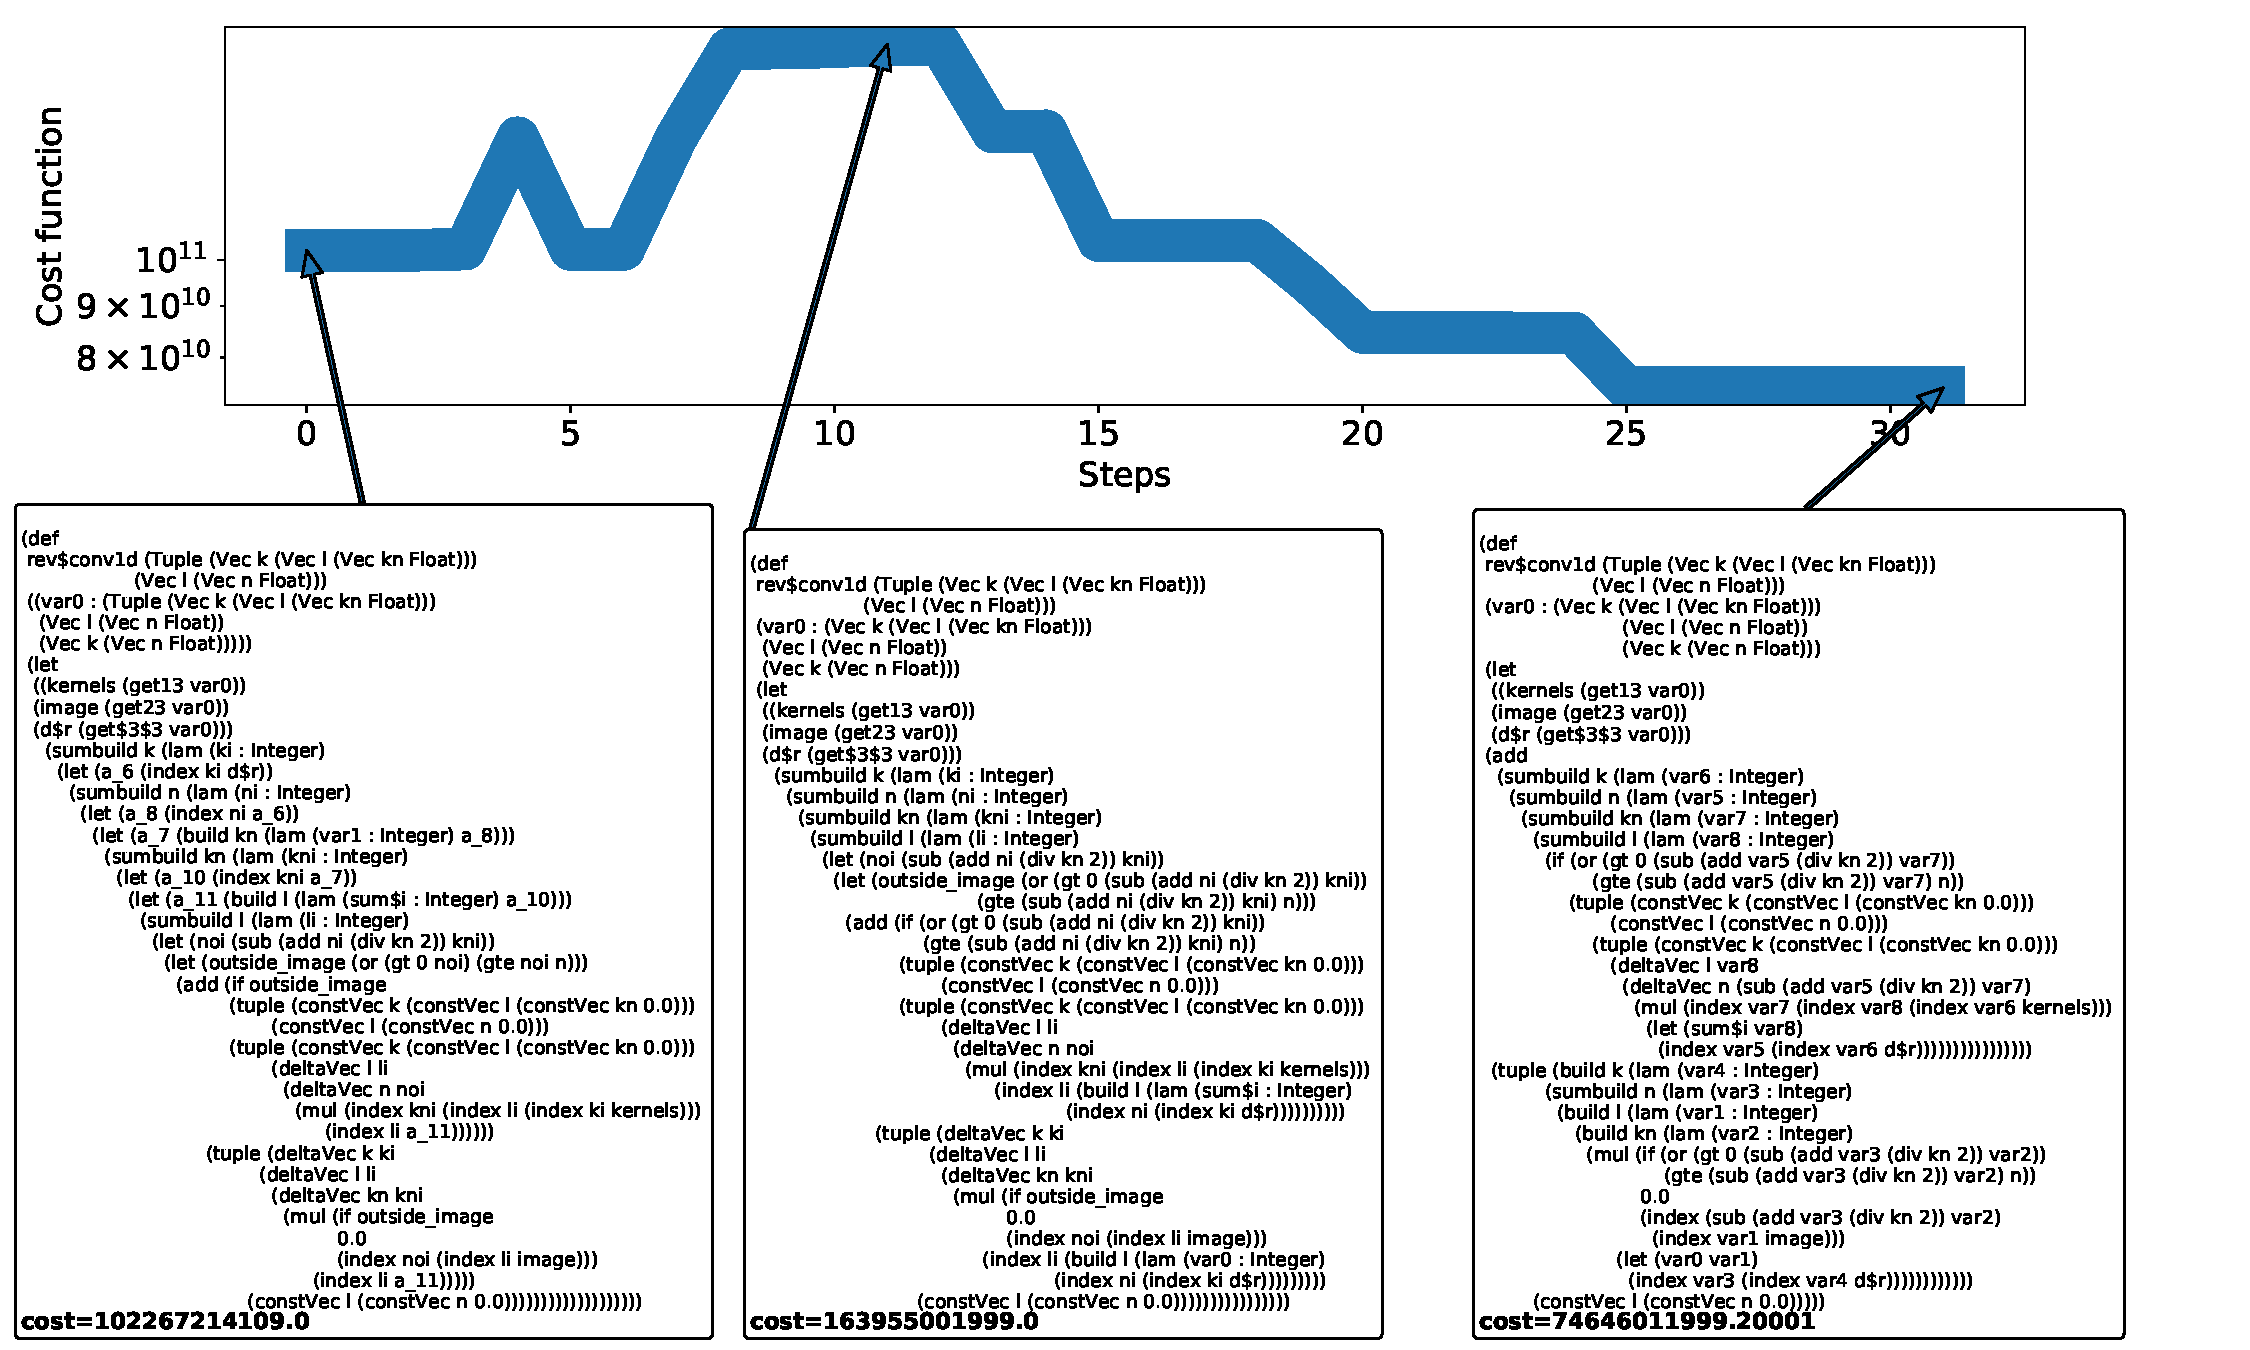
\includegraphics[width=\textwidth]{cost_sequence_mnist.pdf}
  \caption{Reverse mode of convolutional network rewrite sequence obtained by Knossos. The initial expression was obtained from our rule-based \texttt{ksc} compiler and shown in the bottom left. The final expression was obtained after 32 rewriting steps and shown in the bottom right. The expression in the bottom middle corresponds to the highest point in the cost sequence.}
  \label{mnist-qualit}
\end{figure*}


% Finally, in order to asses the performance of the optimizer on more modern workloads, we use Knossos on a computer vision task. We use the VGG16 convolutional deep network \citep{simonyan2014very} and train it on a MNIST dataset \citep{lecun1998mnist}. This allows us to to test the performance of the type-driven automatic differentiation module described in Section \ref{sec-ad} on models with multiple complex layers. The results are shown in Figure \ref{benchmark-dl}. Again, the shaded area represents the standard deviation across the runs of Knossos and the resulting binary. As above, the Knossos optimizer produced code that runs faster than the human baseline.




\paragraph{Summary of Benchmarks}
We have demonstrated that Knossos is capable of producing code that is faster than the output of a traditional compiler. Moreover, unlike traditional compilers, Knossos does not rely on hand-crafted optimisation passes that are very laborious to implement. Instead, traditional optimisation passes are replaced by atomic rewrite rules that can be combined in many ways.
In fact, in our benchmark of linear algebra primitives, Knossos was able to automatically discover \emph{loop fusion}, an optimisation strategy long known to compiler designers. Knossos code in our experiments can perform both training and inference and can be run on any hardware supporting the \Cpp toolchain, including inexpensive embedded devices. 

%(TODO: finalize list of experiments. Other experiments suggested by Andrew: CSAT, bootstrapping i.e. Knossos complies Knossos, TreeNN) 

\section{Conclusions}
We have introduced Knossos, a new compiler targetting machine learning and numerical computation. Thanks to its automatic code optimisation, Knossos produces binaries that achieve better run-times than a traditional, rule-based compiler. Knossos can deal with complex code generated by automatic differentiation and automatically discover  optimisations that previously required careful compiler design. We believe that Knossos will pave the way towards a new generation of future compilers, which will crucially rely on automatically inferring the correct optimisations. 

{
\small
\bibliography{knossos-paper}
\bibliographystyle{iclr2020_conference}
}

\clearpage 
\section*{Appendices}
\renewcommand\thesubsection{Appendix \Alph{subsection}}

\subsection{Knossos Intermediate Representation}
\label{sec:knossos-ir}
\begin{figure}
  \begin{center}
    \begin{minipage}[t]{0.48\textwidth}
  
    \begin{lstlisting}[caption=F\# code for TreeNN, frame=tlrb, language=caml]{knossos_code}
let rec embedding phrase =
  match phrase with
    | Leaf word ->  
       weights.embedding.[word]
    | Node (l,r) ->
       let sl = embedding l (* Recurse left *)
       let sr = embedding r (* Recurse right *)
       tanh (weights.Wl * sl + weights.Wr * sr)
    \end{lstlisting}
    \end{minipage}
    \hspace{0.015\textwidth}
     \begin{minipage}[t]{0.48\textwidth}
    \begin{lstlisting}[caption=TensorFlow code,frame=tlrb,language=python]{tensorflow_code}
def __loop_body(tensor_array, i)
  is_leaf = tf.gather(self.is_leaf_placeholder, i)
  word_index = tf.gather(self.
      word_indices_placeholder, i)
  left_child = tf.gather(self.
      left_children_placeholder, i)
  right_child = tf.gather(self.right_children_placeholder,i)
  node_tensor = tf.cond(is_leaf,
      lambda:__embed_word(word_index),
      lambda:__combine_children(
            tensor_array.read(left_child),
  tensor_array.read(right_child)))
  tensor_array = tensor_array.write(i, node_tensor)
  i= tfadd(i, 1)
  return tensor_array, i
    \end{lstlisting}
    \end{minipage}
  \end{center}
  \caption{Comparison of equivalent code Knossos/F\# vs TensorFlow.}
  \label{fig-comparison}
  \end{figure}
  
For background, we give a brief overview of the intermediate representation (IR) used by the Knossos compiler. the Knossos IR provides a convenient symbolic form for the reinforcement learning optimizer. It also has a LISP-like surface syntax, which we used to implement our programs. In the future, we plan to provide transpilers, allowing for the compilation of code written in other languages into Knossos. We provide a sample Knossos program in Figure \ref{gemm-qualit}.In order to facilitate Machine Learning workloads, the Knossos IL has native support for automatic differentiation. We use a new unified view of automatic differentiation as generalised transposition \citep{elliottSimpleEssenceAutomatic2018}. Rather than having an explicit distinction between forward mode and reverse mode AD, Knossos uses uses a type system together with a set of consistent rewrite rules. Whenever the gradient operator is used as part of a Knossos algorithm, the compiler first generates a syntax tree corresponding to the differentiated program and then applies rewrites to optimize the cost of its execution. This means that the resulting AD algorithm is tailor-made and optimized with that exact use case in mind. This is in contrast to systems such as PyTorch, which have hard-coded routines for backward-mode AD. From the perspective of the user, this process is completely transparent in the sense that taking gradients can be applied to any piece of Knossos code. 

While the details of this process are beyond the scope of this paper, from the perspective of this work, the important feature of AD is that it corresponds to a transformation of the abstract syntax tree. The resulting AST can then be optimised in the same way as any other code.

%For example, to perform supervised learning, one can use the F\# code below.
%\begin{center}
%	\vspace{-1em}
%	\begin{minipage}[t]{0.98\textwidth}
%	\begin{lstlisting}[frame=tlrb]{a}
%weights_trained = adam (w -> loss w examples) weights_init
%	\end{lstlisting}
%	\end{minipage}
%\end{center}
%This calls the adam optimizer, which adjusts the network weights by differentiating the loss. Crucially, {\tt \small  loss} can be an arbitrary F\# function defined in the usual way -- the programmer does not have to know anything about gradients. 



%We provide a transpiler for F\#, effectively giving it automatic differentiation capability. Our system has a modular architecture, meaning that support for additional languages can be added easily. We are already working on a module for Julia. 
  
 %The benefits of our approach are best seen by example. In Figure \ref{fig-comparison}, we compare the same algorithm written in in Knossos with a version written using Python with the TensorFlow library. The code implements a Tree Neural Network and is representative of modern ML workloads.  The TensorFlow code, shown on the right-hand side of Figure \ref{fig-comparison}, follows the \emph{meta-programming} paradigm, where the programmer uses Python to construct a Abstract Syntax Tree (AST), which is then processed with automatic differentiation. Because Python lacks compile-time type safety, logical errors in building up the AST can often be only detected at runtime, making debugging difficult. In fact, some kinds of these errors are so common that special projects have been created to work around them \citep{tensor-considered-harmful}. Some of these errors persist even in Swift for TensorFlow, which is strongly-typed. For example, tensor dimension is not part of the type in Swift for TensorFlow (TODO: does the Knossos type system enforce more constraints, like matrix sizes?).
  
 %The F\# code, shown on the left, follows a more straightforward convention. The programmer simply writes out tree traversal in the normal way. Because of the type systems used in Knossos and F\#, once the code complies, the abstract syntax can be assumed to be free of a broad class of logical errors. Since differentiation in Knossos is a first-class citizen, the programmer can use a short language primitive to perform optimisation with respect to any variable (see Section \ref{sec-ad} for details). This makes writing differentiable programs as easy as writing traditional software while providing all the power of modern machine learning. This technology also makes it possible to use refactoring and other IDE automation tools that already exist for F\#, for differentiable programs, further enhancing programmer productivity. 
  
% Superficially, our approach resembles PyTorch, where the meta-programming is obscured with syntactic sugar such as operator overloading. However, underneath, PyTorch still works by constructing an Abstract Syntax Tree of PyTorch primitives that are fundamentally distinct from Python ones. For example, it means that one cannot import a non-PyTorch Python function and use it in a differentiable PyTorch program. Moreover, because Knossos code is completely decoupled from the source language, it can be easily optimized, allowing for much better performance. 

  




%\paragraph{Arbitrary Tangent Spaces}
%(TODO: this section is aspirational and may not appear in the final paper). Modern deep learning algorithm often involve objects of different types. For example, algorithms that perform probabilistic modelling use probability distributions, while algorithms that manipulate 3D rotations might use quaternions. Even though both are ultimately represented as vectors of real numbers, comparing them by simply computing the Euclidean distance between these vectors does not reflect their properties. Instead, one should use a notion of similarity that is tailor-made for a specific type of object \citep{deza2009encyclopedia}. For example, the natural way to compare probability distributions is to use an $\alpha$-divergence while the natural way to compare quaternions is to use an elliptic distance. This notion of similarity becomes crucial when defining gradients. Since a gradient quantifies the behaviour of a function in a small neighbourhood of its argument, it is critical that this neighbourhood is defined using the right notion of similarity. Each type of similarity corresponds to a specific way of computing the gradients, known as the tangent space. 
%
%The Knossos type system supports arbitrary tangent spaces natively. For example, in Knossos, all that is needed to turn a regular policy gradient algorithm (which compares policies using their parameters) into a natural policy gradient algorithm (which compares policies using the KL-divergence) is to declare that the policy object is of type \emph{probability distribution}. For example,
%\begin{center}
%	{\tt \small pi$\,$:$\,$Vector<double>} becomes { \tt \small pi$\,$:$\,$Multinomial} . 
%\end{center}
%Since Knossos compares probability distributions using the KL divergence by default, using natural gradients is trivial.

\subsection{Reproducibility and Details of Experimental Setup}
\label{sec:exp-setup}
We now describe the parameters used to perform the experiments reported on in the paper. The parameters used by $A^\star$ in the four tasks described in Sec.~\ref{sec-benchmarks} are listed in Tab.~\ref{tbl:benchmarks}. The hyper-parameters for the value network training are given in Tab.~\ref{tbl:hyperparameters}.

\begin{table}
    \centering
    \caption{List of Experimental Settings}
    \begin{tabular}{ll}
      \toprule
      \multicolumn{2}{c}{Arithmetic Expressions} \\
      {\bf Parameter}                              &  {\bf Value} \\ \midrule
      Number of training expressions               & 36 \\
      Number of test expressions                   & 12 \\
      Rewrite rules                                & Simple rule set \\
      Number of evaluation budget per epoch        & 5000 \\
      Minimum batch size for evaluation            & 16 \\
      Maximum Search Depth                         & 10 \\
      \multicolumn{2}{c}{Basic Linear Algebra} \\ \midrule
      Number of training expressions               & 11 \\
      Number of test expressions                   & 1 \\
      Rewrite rules                                & Extended rule set \\
      Number of evaluation budget per epoch        & 30000 \\
      Minimum batch size for evaluation            & 16 \\
      Maximum Search Depth                         & 30 \\
    %   \multicolumn{2}{c}{Gaussian Mixture Model} \\ \midrule
    %   Number of training expressions               & TODO \\
    %   Number of test expressions                   & TODO \\
    %   Rewrite rules                                & Extended rule set \\
    %   Number of evaluation budget per epoch        & 30000 \\
    %   Minimum batch size for evaluation            & 16 \\
    %   Maximum Search Depth                         & 30 \\
      \multicolumn{2}{c}{Convolutional Neural Network} \\ \midrule
      Number of training expressions               & 5 \\
      Number of test expressions                   & 1 \\
      Rewrite rules                                & Extended rule set \\
      Number of evaluation budget per epoch        & 30000 \\
      Minimum batch size for evaluation            & 16 \\
      Maximum Search Depth                         & 40 \\ \midrule
      
      \bottomrule
    \end{tabular}
    \label{tbl:benchmarks}
  \end{table}
  %\todo{Batch size only appears in this table.}

\begin{table}
  \centering
  \caption{List of hyperparameters}
  \begin{tabular}{ll}
    \toprule
    % \multicolumn{2}{c}{{\bf Deep $A^\star$ Search}} \\
    % {\bf Parameter}                        &  {\bf Value} \\ \midrule
    % Minimum batch size for evaluation            & 16 \\ \midrule
    % \\
    \multicolumn{2}{c}{{\bf Value Function}} \\
    {\bf Model Parameter}                        & \\ \midrule
    Number of features per node                  & 200 \\
    Number of propagation steps                  & 10 \\
    Activation function for GNN                  & tanh \\
    Dropout rate for GNN                         & 0 \\
    Number of hidden layers in MLP               & 2 \\
    Hidden layer dimensionality & 200 \\    
    Activation function for MLP                  & tanh \\
    Dropout rate for MLP                         & 0.2 \\
    \\
    {\bf Training Parameter}                     &  \\
    Loss function                                & Huber loss \\
    Optimizer                                    & Adam  \\
    Learning rate                                & 0.0001 \\
    Batch size                                   & 16 \\
    \bottomrule
  \end{tabular}
  \label{tbl:hyperparameters}
\end{table}

In the Graph Neural Network, initial node features are one-hot vectors that represent the node types. The used node types are: {constant, variable, let, if, tuple, select, +, -, *, /, exp, log, $==$, $>$, $>=$, or, build, apply, lam, sum, sumbuild, constVec, and deltaVec}.
%
Edge types are listed in Tab.~\ref{tab:edge-types}. The auxiliary edge type``is-identical'' is inserted to identify identical subexpressions. It was added so that it is easier to learn re-writes that rely on matching expressions. % \todo[inline]{TODO: cite paper using matching-edge}. % I think it's fine not to cite it because people are using it without citing it.
The GNN was implemented using a sparse adjacency matrix instead of dense matrix in order to conserve GPU memory in settings where some expressions grow beyond $>10000$ nodes during training. We ran the GNN recursion 10 times.  For optimization we used the Adam optimizer with learning rate $0.0001$ and set the dropout rate zero for GNN and 0.2 for the MLP.
% We use edge types as edge features and do not learn edge embedding.
%



\subsection{Rewrite rules}
\label{appendix-rewrites}
We list the basic rule set used in the arithmetic expressions benchmark in Tab.~\ref{tbl:rules}. The additional rewrite rules used in basic linear algebra and convolutional neural network are given in Tab.~\ref{tbl:extended_rules}.

\begin{table*}
  \centering
  \caption{List of rewrite rules used for arithmetic expressions.}
  \begin{tabular}{lll}
    \toprule
        \multicolumn{3}{c}{{\bf Simple Rule Set}} \\
        {\bf LHS}                        &  {\bf RHS}                  & {\bf Side conditions} \\ \midrule
       \multicolumn{3}{c}{{\bf Arithmetic Rules}} \\
       
 (add 0.0 a) & a \\
 (mul 1.0 a) & a \\
 (sub a 0.0) & a \\
 (div a 1.0) & a \\
 (add a (mul b -1.0)) & (sub a b) \\
 (mul a b) & (mul b a) \\
 (add a b) & (add b a) \\
 (sub a a) & 0.0 \\
 (add (add a b) c) & (add (add a c) b) \\
 (sub (add a b) c) & (add (sub a c) b) \\
 (add (sub a b) c) & (sub (add a c) b) \\
 (sub (sub a b) c) & (sub (sub a c) b) \\
 (sub a (sub b c)) & (sub (add a c) b) \\
 (mul (mul a b) c) & (mul (mul a c) b) \\
 (div (mul a b) c) & (mul (div a c) b) \\
 (mul (div a b) c) & (div (mul a c) b) \\
 (div (div a b) c) & (div (div a c) b) \\
 (div a (div b c)) & (div (mul a c) b) \\
 (div (div a b) c) & (div a (mul b c)) \\
 (mul a (add b c)) & (add (mul a b) (mul a c)) \\
 (add (mul a b) (mul a c)) & (mul a (add b c)) \\
 (mul a (sub b c)) & (sub (mul a b) (mul a c)) \\
 (add a (mul -1.0 b)) & (sub a b) \\
 (sub (mul a b) (mul a c)) & (mul a (sub b c)) \\
 (add (div y x) (div z x)) & (div (add y z) x) \\
 (sub (div y x) (div z x)) & (div (sub y z) x) \\
 (div a (mul b c)) & (div (div a b) c) \\
 (mul 0.0 a) & 0.0 \\
       \multicolumn{3}{c}{{\bf Binding Rules}} \\
        e & (let (x e) x) \\ 
        (op (let (x e) x)) & (let (x e) (op x)) & x $\notin$ op \\
        (let (x e1) (let (x e1) e2)) & (let (x e1) e2) \\
        (let (x e1) e2) & (let (x e1) e2[x/e1]) & replace all free x in e2 with e1 \\
        (let (x e1) e2) & e2 & x $\notin$ e2 \\
   \bottomrule
  \end{tabular}
  \label{tbl:rules}
\end{table*}
        
\begin{table*}
  \caption{List of rewrite rules used in addition to simple rule set (Table \ref{tbl:rules}) for Basic Linear Algebra and Convolutional Neural Network benchmarks. In the two-phase strategy described in Sec.~\ref{sec-benchmarks}, only the rules with checkmarks in the last column are used for the first 15 epochs.}
  \adjustbox{max width=\textwidth}{
  \centering
  \begin{tabular}{llll}
    \toprule
        \multicolumn{3}{c}{{\bf Extended Rule Set}} \\
        {\bf LHS}                        &  {\bf RHS}                  & {\bf Side conditions} & {\bf Include in phase 1} \\ \midrule
        %\multicolumn{3}{c}{{\bf Build Rules}} \\
        (size (build n (lam x b))) & n \\
        (index arg (build sz (lam x body))) & (let (x arg) body) & & \checkmark \\
        (select i (tuple e1 e2 e3...)) & ei \\
        (sum (build n (lam x b))) & (sumbuild n (lam x b))  & & \checkmark \\
        (sumbuild n (lam x (deltaVec m i v))) & (deltaVec m i (sumbuild n (lam x v))) &  x$\notin$ m $\cap$ x $\notin$ i. & \checkmark \\
        (sumbuild n (lam x (tuple f g))) & (tuple (sumbuild n (lam x f)) (sumbuild n (lam x g))) & & \checkmark \\
        (sumbuild n (lam x (if c t f))) & (if c (sumbuild n (lam x t)) (sumbuild n (lam x f))) & & \checkmark \\
        (sumbuild n (lam x c)) & (mul n c) & x $\notin$ c $\cap$ c is a constant & \checkmark \\
        (sumbuild o (lam oi (add e1 e2))) & (add (sumbuild o (lam oi e1)) (sumbuild o (lam oi e2))) & & \checkmark \\
        (sumbuild o (lam oi (build n (lam ni e)))) & (build n (lam ni (sumbuild o (lam oi e)))) & & \checkmark \\
        (add (deltaVec o oi e1) (deltaVec o oi e2)) & (deltaVec o oi (add e1 e2)) & & \checkmark \\
        (add (tuple x y) (tuple a b)) & (tuple (add x a) (add y b)) & & \checkmark\\
        (mul (tuple x y) z) & (tuple (mul x z) (mul y z)) & & \checkmark\\
        %\multicolumn{3}{c}{{\bf If Rules}} \\
        (if True a b) & a \\
        (if False a b) & b \\
        (if p True False) & p \\
        (if p a a) & a \\
        (eq a a) & True & \\
    \bottomrule
  \end{tabular}
  }
  \label{tbl:extended_rules}
\end{table*}


\subsection{Additional  ablations.}
\label{ablation-mcts}
% MCTS is a common reinforcement learning technique applied to combinatorial optimization problems \cite{kaliszykReinforcementLearningTheorem2018,Silver2016}.
In addition to $A^\star$ search, we compare the performance of Monte Carlo Tree Search \citep{browne2012survey} using the UCT formula \citep{auer2002finite,kocsis2006bandit}. In order to disambiguate across subtly different versions of the algorithm, we describe it below.

Each iteration of MCTS consists of four steps (Algorithm \ref{lst:mcts}).
\begin{enumerate}
    \item Selection: Starting from the root, a tree policy is recursively descends through the tree until it reaches a leaf node.
    \item Expansion: A child node is added to expand the tree.
    \item Simulation: A rollout policy is applied from the new node until the end of the episode.
    \item Back-up: The simulation result is backed up through the selected nodes to update their statistic.
\end{enumerate}

The tree policy $\pi_t$ and rollout policy $\pi_r$ are defined as follows.

\begin{align}
    \pi_t(a | s) &= \textstyle \argmax_{a \in A}\left( \frac{X(s')}{n(s')} + \beta \sqrt{ \frac{\ln n(s)}{n(s') + 1}} \right) \\
    \pi_r(a | s) &= \text{softmax}_{a \in A}( R(s, a) + V(s'), \alpha)
\end{align}

Here, $n(s)$ is a visitation count of state $s$, and $\beta$ is a constant to control the exploration bonus. $X(s') / n(s')$ is the average cost reduction achieved by a set of trajectories which passed through $s'$ in $M$: $X(s') = \sum_{T \in H : s' \in T} \max_{s_d \in T : d(s_d) \geq d(s')} c(s_0) - c(s_d)$, and $M$ is a set of trajectories sampled at current epoch for the current expression so far. The more the state $s'$ is visited, the exploration bonus $(\beta \sqrt{ \frac{\ln n(s)}{n(s') + 1}})$ is reduced. This way, the agent is encouraged to try a diverse set of actions.


\begin{algorithm}[t]
\caption{Monte Carlo Tree Search (MCTS)}
\begin{algorithmic}
%    \Function {MCTS-Init}{$s_0$, $V$, $d$, $\alpha$, $c$}
%    \State $\pi_t(a|s) \leftarrow \argmax_{a \in A}( X(s') / n(s') + c \sqrt{ \frac{\ln n(s)}{n(s') + 1}})$
%    \State $\pi_r(a|s) \leftarrow \text{softmax}_{a \in A}( R(s, a) + V(s'), \alpha)$
%    \State \Return MCTS($s_0$, $d$, $\pi_t$, $\pi_r$)
%    \EndFunction
%    \\
    \Function {MCTS}{$s_0$, $V$, $d$, $\alpha$, $c$}
    \State $\pi_t(a|s) \leftarrow \argmax_{a \in A}\left( X(s') / n(s') + \beta \sqrt{ \frac{\ln n(s)}{n(s') + 1}} \right)$
    \State $\pi_r(a|s) \leftarrow \text{softmax}_{a \in A}( R(s, a) + V(s'), \alpha)$
    
    \State $M \leftarrow \emptyset$
    \State $\forall s \in S: n(s) \leftarrow 0$ \Comment{Initialize a visitation count}
    \While {{\bf not} term\_condition$()$}
        \State $T_t \leftarrow \textsc{TreeSearch}(s_0, d, \pi_t)$
        \State $s_l \leftarrow \text{tail}(T_t)$
        % \State $n(s_l) \leftarrow n(s_l) + 1$
        \State $T_r \leftarrow \textsc{RolloutSearch}(s_l, d - \text{length}(T_t), \pi_r)$
        \State $T \leftarrow \text{concat}([s_0], T_t, T_r)$
        \State $x \leftarrow c(s_0) - \min_{s \in T_r} c(s)$ 
        % \State $x \leftarrow \max_{s \in T_r}  R(s, \pi(s))$ 
        \LineComment{$x$ is the max cost reduction found by rollout}
        \ForAll {$s \in T_t$}
            \Comment{MCTS backup}
            \State $X(s) \leftarrow X(s) + x$
            \State $n(s) \leftarrow n(s) + 1$
        \EndFor
        \State $M \leftarrow M \cup \{T\}$
    \EndWhile
    \State \Return $M$
    \EndFunction
    \\
    \Function {TreeSearch}{$s$, $d$, $\pi$}
        \State $T \leftarrow []$
        \While {$\text{length}(T) < d$ \textbf{ and } $n(s) > 0$}
            % \State $n(s) \leftarrow n(s) + 1$
            \State $a \leftarrow \pi(a | s)$ \Comment{Tree policy $\pi$ is deterministic.}
            \State $s \leftarrow a \circ s$
            \State $T \leftarrow \text{concat}(T, [s])$      
        \EndWhile
        \State \Return $T$
    \EndFunction
\end{algorithmic}
\label{lst:mcts}
\end{algorithm}


We evaluated the performance of $A^\star$ search and MCTS for both training and test. The experimental setup is the same as the \emph{Generalisation to Unseen Data} experiment in Section \ref{sec-benchmarks} except for the used  search algorithm. For MCTS, we used $\alpha=5.0$ and $\beta=0.5$ for both training and test. 

Figure \ref{fig:train-comparison} shows the results of running all possible combinations of search algorithms when used for training and test in various configurations. Overall, using $A\star$ for both training and test achieved the best performance. In particular, when we fixed the algorithm used during test to $A^\star$ and varied the training algorithm between $A^\star$ and MCTS, $A\star$ achieved a significantly lower the total minimum cost than MCTS. Similarly, when we fixed the algorithm used for training to $A\star$ and compared the performance during testing $A\star$ achieved significantly lower cost than MCTS again.

\begin{figure*}[t!]
	\centering
  	\begin{subfigure}[t]{0.33\textwidth}
  		\centering
	    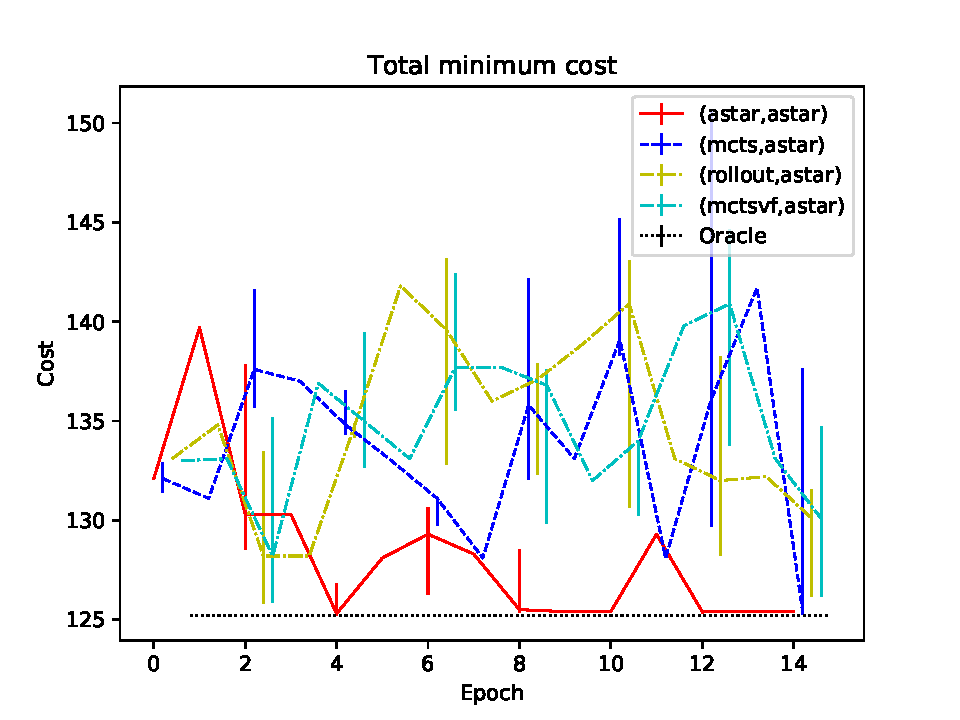
\includegraphics[width=\textwidth]{generalization-train-compare.pdf}
	    \caption{Generalization (Train)}
	    \label{fig:train-comparison}
	\end{subfigure}%
  	\begin{subfigure}[t]{0.33\textwidth}
  		\centering
	    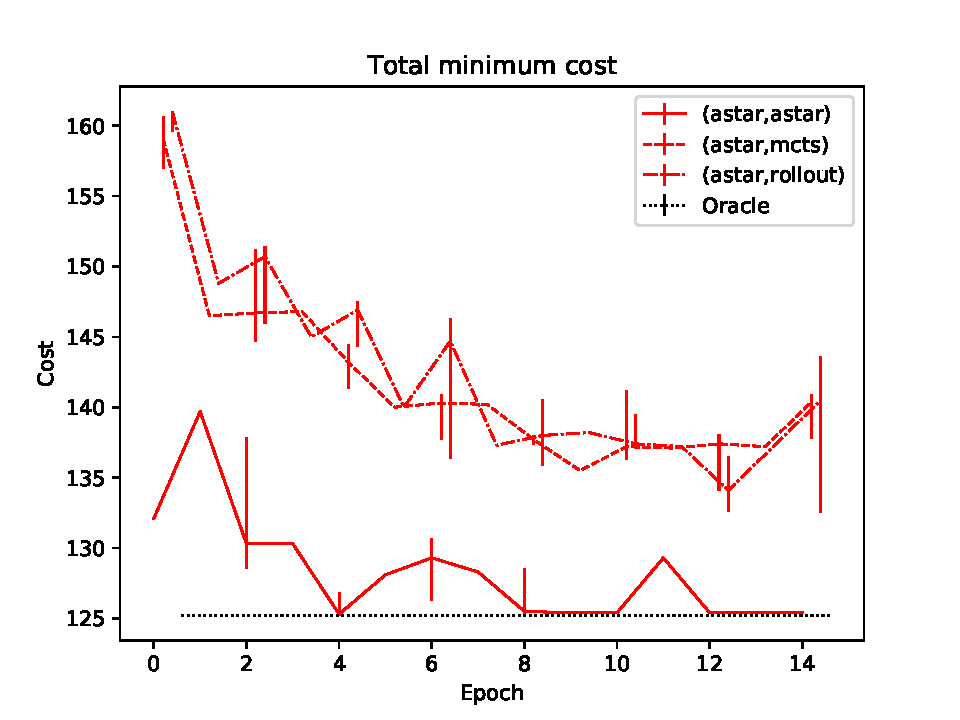
\includegraphics[width=\textwidth]{generalization-test-compare.pdf}
	    \caption{Generalization (Test)}
	    \label{fig:test-comparison}
	\end{subfigure}
  	\begin{subfigure}[t]{0.33\textwidth}
  		\centering
	    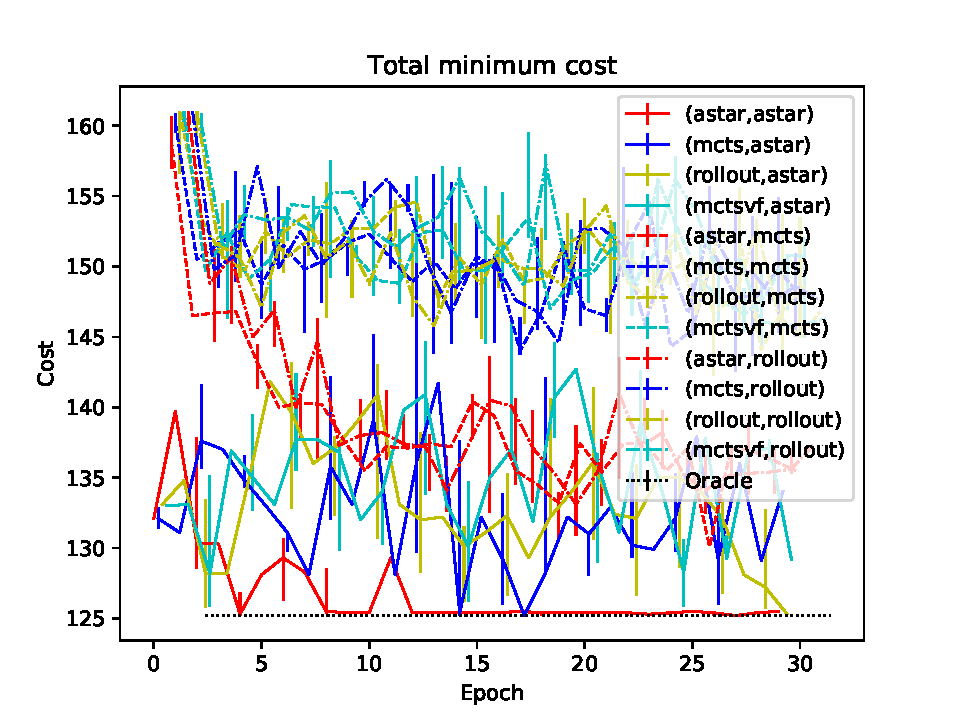
\includegraphics[width=\textwidth]{generalization-compare.pdf}
	    \caption{Generalization}
	    \label{fig:comparison}
	\end{subfigure}
    \caption{Comparison of $A\star$ search and Monte Carlo Tree Search.}
    \label{benchmark-arithmetic}
\end{figure*}



\subsection{List of Expressions}

\begin{table*}
  \centering
  \caption{List of expressions for Generalization to Unseen Expressions.}
  \begin{tabular}{l}
  \toprule
          \multicolumn{1}{c}{{\bf Train expression set}} \\ \midrule
(mul (div (mul 2.0 (add x y)) (sub (add x y) 1)) (mul x y))  \\
(add (add (mul x 2.0) 1) (div (add (div x (sub y 1)) (mul x 2.0)) 2))  \\
(div (add (mul 2.0 (mul x y)) (mul x y)) (div 1.0 (add x 1)))  \\
(div (add (add (div x (sub y 1)) (log x)) 1) (sub (mul (div x (sub y 1)) 3) 1))  \\
(add (div (div 1.0 (add x 1)) (add (add x y) (div 1.0 (add x 1)))) (div 1.0 (add x 1)))  \\
(mul (add (log x) (mul x 2.0)) (mul (log x) 3))  \\
(mul (add (add x y) (log x)) (mul (add x y) 3))  \\
(div (add (add (mul x 2.0) 1) 1) (sub (add (add x y) (mul x 2.0)) 1))  \\
(sub (mul (mul 2.0 (mul x y)) (mul x y)) (mul x 2.0))  \\
(mul (add (div x (sub y 1)) 1) (add (mul x y) (div x (sub y 1))))  \\
(mul (div (div 1.0 (add x 1)) (add (div x (sub y 1)) (div 1.0 (add x 1)))) (div 1.0 (add x 1)))  \\
(add (add (log x) (div 1.0 (add x 1))) (div (mul (log x) 3) 2))  \\
(add (add (add x y) (div x (sub y 1))) (div (mul (add x y) 3) 2))  \\
(div (mul (mul x 2.0) (mul x 2.0)) (sub (mul x 2.0) (div 1.0 (add x 1))))  \\
(mul (div (mul 2.0 (mul x y)) (sub (mul x y) 1)) (log x))  \\
(add (add (div x (sub y 1)) 1) (div (add (add x y) (div x (sub y 1))) 2))  \\
(div (add (mul 2.0 (div 1.0 (add x 1))) (div 1.0 (add x 1))) (mul x 2.0))  \\
(div (add (add (log x) (mul x y)) 1) (sub (mul (log x) 3) 1))  \\
(div (add (add (add x y) (mul x 2.0)) 1) (sub (mul (add x y) 3) 1))  \\
(add (div (mul x 2.0) (add (mul x y) (mul x 2.0))) (mul x 2.0))  \\
(mul (add (mul x y) (div x (sub y 1))) (mul (mul x y) 3))  \\
(div (add (add (div x (sub y 1)) 1) 1) (sub (add (div 1.0 (add x 1)) (div x (sub y 1))) 1))  \\
(sub (mul (mul 2.0 (div 1.0 (add x 1))) (div 1.0 (add x 1))) (log x))  \\
(mul (add (log x) 1) (add (add x y) (log x)))  \\
(mul (add (add x y) 1) (add (div 1.0 (add x 1)) (add x y)))  \\
(mul (div (mul x 2.0) (add (log x) (mul x 2.0))) (mul x 2.0))  \\
(add (add (mul x y) (add x y)) (div (mul (mul x y) 3) 2))  \\
(div (mul (div x (sub y 1)) (div x (sub y 1))) (sub (div x (sub y 1)) (mul x 2.0)))  \\
(mul (div (mul 2.0 (div 1.0 (add x 1))) (sub (div 1.0 (add x 1)) 1)) (mul x y))  \\
(add (add (log x) 1) (div (add (div x (sub y 1)) (log x)) 2))  \\
(add (add (add x y) 1) (div (add (mul x y) (add x y)) 2))  \\
(div (add (mul 2.0 (mul x 2.0)) (mul x 2.0)) (div x (sub y 1)))  \\
(div (add (add (mul x y) (div 1.0 (add x 1))) 1) (sub (mul (mul x y) 3) 1))  \\
(add (div (div x (sub y 1)) (add (log x) (div x (sub y 1)))) (div x (sub y 1)))  \\
(mul (add (div 1.0 (add x 1)) (add x y)) (mul (div 1.0 (add x 1)) 3))  \\
(div (add (add (log x) 1) 1) (sub (add (mul x 2.0) (log x)) 1))  \\ \midrule
        \multicolumn{1}{c}{{\bf Test expression set}} \\ \midrule
(div (add (mul 2.0 (add x y)) (add x y)) (mul x 2.0))  \\
(div (add (add (mul x 2.0) (mul x y)) 1) (sub (mul (mul x 2.0) 3) 1))  \\
(add (div (mul x y) (add (div x (sub y 1)) (mul x y))) (mul x y))  \\
(mul (add (div x (sub y 1)) (div 1.0 (add x 1))) (mul (div x (sub y 1)) 3))  \\
(div (add (add (div 1.0 (add x 1)) 1) 1) (sub (add (log x) (div 1.0 (add x 1))) 1))  \\
(sub (mul (mul 2.0 (log x)) (log x)) (add x y))  \\
(sub (mul (mul 2.0 (add x y)) (add x y)) (div 1.0 (add x 1)))  \\
(mul (add (mul x 2.0) 1) (add (log x) (mul x 2.0)))  \\
(mul (div (mul x y) (add (add x y) (mul x y))) (mul x y))  \\
(add (add (div x (sub y 1)) (mul x 2.0)) (div (mul (div x (sub y 1)) 3) 2))  \\
(div (mul (div 1.0 (add x 1)) (div 1.0 (add x 1))) (sub (div 1.0 (add x 1)) (mul x y)))  \\
(mul (div (mul 2.0 (log x)) (sub (log x) 1)) (div x (sub y 1)))  \\
\bottomrule
  \end{tabular}
  \label{tbl:generalization-expressions}
\end{table*}

\begin{table*}
  \centering
  \caption{List of expressions for Generalization scenario.}
  \begin{tabular}{l}
  \toprule
        \multicolumn{1}{c}{{\bf Train/Test expression set}} \\ \midrule
(div (div 1.0 x) (add 1.0 (div 1.0 x)))  \\
(add (div (div 1.0 x) (add (div 1.0 x) 1.0)) (div 1.0 x))  \\
(add (div (div 1.0 x) (add (div 1.0 x) 2.0)) (div 1.0 x))  \\
(mul (div x y) (div x y))  \\
(div (mul (div x y) x) y)  \\
(add (div (mul x y) (add 1.0 (mul x y))) (mul x y))  \\
(add (div 1.0 (add 1.0 (mul x y))) (mul x y))  \\
(div (mul x y) (add 1.0 (mul x y)))  \\
  \bottomrule
  \end{tabular}
  \label{tbl:standard-expressions}
\end{table*}
        
\begin{figure*}
  \centering
  \caption{List of expressions in training set for Linear Algebra Primitives.}
  \adjustbox{max width=\textwidth}{
  \begin{lstlisting}{blas-train}
(def
 float_matrix_multiply (Vec n (Vec m Float))
 ((alpha : Float) (mat_x : Vec n (Vec m Float)))
 (build n
        (lam (i : Integer) (build m
                                  (lam (j : Integer) (mul alpha (index i (index j mat_x))))))))
(def
 matrix_matrix_multiply (Vec n (Vec l Float))
 ((mat_x : Vec n (Vec m Float)) (mat_y : Vec m (Vec l Float)))
 (build n
  (lam (i : Integer) (build l
    (lam (k : Integer) (sumbuild m
      (lam (j : Integer) (mul (index i
                                      (index j
                                       mat_x))
                                     (index j
                                      (index k
                                       mat_y))))))))))
(def
 vector_vector_add (Vec n Float)
 ((vec_x : Vec n Float) (vec_y : Vec n Float))
 (build n (lam (i : Integer) (add (index i vec_x) (index i vec_y)))))
(def
 matrix_matrix_add (Vec n (Vec m Float))
 ((mat_x : Vec n (Vec m Float)) (mat_y : Vec n (Vec m Float)))
 (build n
        (lam (i : Integer) (build m
                                  (lam (j : Integer) (add (index i (index j mat_x))
                                                        (index i (index j mat_y))))))))
(def
 outer_product (Vec n (Vec m Float))
 ((vec_x : Vec n Float) (vec_y : Vec m Float))
 (build n
        (lam (i : Integer) (build m
                                  (lam (j : Integer) (mul (index i vec_x) (index j vec_y)))))))
(def
 transpose (Vec m (Vec n Float))
 ((mat_x : Vec n (Vec m Float)))
 (build m
        (lam (i : Integer) (build n
                                  (lam (j : Integer) (index j (index i mat_x)))))))
(def
 scal (Vec n Float)
 ((a : Float) (vec_x : Vec n Float))
 (build n (lam (i : Integer) (mul a (index i vec_x)))))
(def
 axpy (Vec n Float)
 ((alpha : Float) (vec_x : Vec n Float) (vec_y : Vec n Float))
 (build n
        (lam (i : Integer) (add (index i (scal alpha vec_x))
                              (index i vec_y)))))
(def
 dot Float
 ((vec_x : Vec n Float) (vec_y : Vec n Float))
 (sumbuild n
           (lam (i : Integer) (mul (index i vec_x) (index i vec_y)))))
(def
 rscl (Vec n Float)
 ((vec_x : Vec n Float))
 (build n (lam (i : Integer) (div (index i vec_x) (sum vec_x)))))
(def
 rot (Tuple (Vec n Float) (Vec n Float))
 ((x : Vec n Float) (y : Vec n Float) (c : Float) (s : Float))
 (tuple (build n
               (lam (i : Integer) (add (mul c (index i x)) (mul s (index i y)))))
        (build n
               (lam (i : Integer) (add (mul (mul -1.0 s) (index i x))
                                     (mul c (index i y)))))))
  \end{lstlisting}
}
\end{figure*}

\begin{figure*}
  \centering
  \caption{Test expression for Linear Algebra Primitives (General Matrix Multiplication).}
  \adjustbox{max width=\textwidth}{
  \begin{lstlisting}{blas-test}
(def
 gemm (Vec n (Vec l Float))
 ((var0 : (Tuple Float
                 (Vec n (Vec m Float))
                 (Vec m (Vec l Float))
                 Float
                 (Vec n (Vec l Float)))))
 (let (beta (get$4$5 var0))
 (let (mat_b (get$3$5 var0))
 (let (mat_a (get$2$5 var0))
 (let (alpha (get$1$5 var0))
 (let (mat_c (get$5$5 var0))          
   (let (mat_x (build n (lam (var4 : Integer)
                 (build l (lam (k : Integer)
                   (sumbuild m (lam (var5 : Integer)
                     (mul (index var4 (index var5 mat_a))
                          (index var5 (index k mat_b))))))))))
   (let (mat_x_6 (build n (lam (var2 : Integer)
                   (build m (lam (var3 : Integer)
                     (mul alpha (index var2 (index var3 mat_x))))))))
   (let (mat_y (build n (lam (var6 : Integer)
                 (build m (lam (var1 : Integer)
                   (mul beta (index var6 (index var1 mat_c))))))))
           (build n (lam (i : Integer)
             (build m (lam (j : Integer)
               (add (index i (index j mat_x_6))
                    (index i (index j mat_y)))))))))))))))
   \end{lstlisting}
}
\end{figure*}

\begin{figure*}
  \centering
  \caption{List of expressions in training set for conv1d.}
  \adjustbox{max width=\textwidth}{
  \begin{lstlisting}{cnn-train}
(def
 rev$matrix_multiply (Tuple (Vec o (Vec k Float)) (Vec k Float))
 ((w : Vec o (Vec k Float))
  (image : Vec k Float)
  (d$r : Vec o Float))
 (sumbuild o (lam (oi : Integer)
  (let ((a_6 (index oi d$r))
        (a_5 (build k (lam (sum$i : Integer) a_6))))
       (tuple (sumbuild k (lam (ki : Integer)
                  (deltaVec o oi
                   (deltaVec k ki
                     (mul (index ki image) (index ki a_5))))))
               (build k (lam (ki : Integer)
                 (mul (index ki (index oi w)) (index ki a_5)))))))))
(def
 rev$matrix_multiply_transpose (Tuple (Vec k (Vec o Float))
                                      (Vec k Float))
 ((w : Vec k (Vec o Float))
  (image : Vec k Float)
  (d$r : Vec o Float))
 (sumbuild o (lam (oi : Integer)
   (let ((a_6 (index oi d$r))
          (a_5 (build k (lam (sum$i : Integer) a_6))))
        (tuple (build k (lam (ki : Integer)
                  (deltaVec o oi
                   (mul (index ki image) (index ki a_5)))))
                 (build k (lam (ki : Integer)
                   (mul (index oi (index ki w)) (index ki a_5)))))))))
(def
 rev$max_ (Tuple Float Float)
 ((x1 : Float) (x2 : Float) (d$r : Float))
 (if (gt x1 x2) (tuple d$r 0.0) (tuple 0.0 d$r)))
(def
 rev$maxpool (Vec n Float)
 ((image : Vec n Float) (d$r : Vec m Float))
 (sumbuild (div n 2) (lam (ni : Integer)
   (let  ((t1698 (mul 2 ni))
          (t1702 (add 1 t1698))
          (t1705 (rev$max_ (index t1698 image)
                                   (index t1702 image)
                                   (index ni d$r))))
        (add (deltaVec n t1698 (select t1705 0))
               (deltaVec n t1702 (select t1705 1)))))))
(def
 rev$expensive (Tuple Float Float)
 ((x1 : Float) (x2 : Float) (d$r : Float))
 (tuple 0.0 0.0))
(def
 rev$expensivepool (Vec n Float)
 ((image : Vec n Float) (d$r : Vec m Float))
 (sumbuild (div n 2) (lam (ni : Integer)
   (let ((t1720 (mul 2 ni))
         (t1724 (add 1 t1720))
         (t1727 (rev$expensive (index t1720 image)
                                        (index t1724 image)
                                        (index ni d$r))))
        (add (deltaVec n t1720 (select t1727 0))
               (deltaVec n t1724 (select t1727 1)))))))
 \end{lstlisting}
}
\end{figure*}

\begin{figure*}
  \centering
  \caption{Test expression for Convolutional Network.}
  \adjustbox{max width=\textwidth}{
  \begin{lstlisting}{cnn-train}
(def
 rev$conv1d (Tuple (Vec k (Vec l (Vec kn Float))) 
                   (Vec l (Vec n Float)))
 ((var0 : (Tuple (Vec k (Vec l (Vec kn Float)))
   (Vec l (Vec n Float))
   (Vec k (Vec n Float)))))
 (let
  ((kernels (get$1$3 var0))
  (image (get$2$3 var0))
  (d$r (get$3$3 var0)))
    (sumbuild k (lam (ki : Integer) 
      (let (a_6 (index ki d$r)) 
        (sumbuild n (lam (ni : Integer) 
          (let (a_8 (index ni a_6)) 
            (let (a_7 (build kn (lam (var1 : Integer) a_8))) 
              (sumbuild kn (lam (kni : Integer) 
                (let (a_10 (index kni a_7)) 
                  (let (a_11 (build l (lam (sum$i : Integer) a_10))) 
                    (sumbuild l (lam (li : Integer) 
                      (let (noi (sub (add ni (div kn 2)) kni)) 
                        (let (outside_image (or (gt 0 noi) (gte noi n))) 
                          (add (if outside_image 
                                   (tuple (constVec k (constVec l (constVec kn 0.0)))
                                          (constVec l (constVec n 0.0))) 
                                   (tuple (constVec k (constVec l (constVec kn 0.0))) 
                                          (deltaVec l li 
                                            (deltaVec n noi 
                                              (mul (index kni (index li (index ki kernels))) 
                                                   (index li a_11)))))) 
                               (tuple (deltaVec k ki 
                                        (deltaVec l li 
                                          (deltaVec kn kni 
                                            (mul (if outside_image 
                                                     0.0 
                                                     (index noi (index li image))) 
                                                 (index li a_11))))) 
                                      (constVec l (constVec n 0.0)))))))))))))))))))
  \end{lstlisting}
}
\end{figure*}
\end{document}
